\documentclass[11pt, a4paper]{article}

\usepackage[utf8]{inputenc}
\usepackage[T1]{fontenc}
\usepackage{amsmath, amssymb} % Math packages
\usepackage{graphicx}        % For including images
\usepackage[margin=1in]{geometry} % Sensible margins
\usepackage{hyperref}        % For potential links (optional)
\usepackage{xcolor}          % For color definitions (used minimally)
\usepackage{caption}         % Better control over captions
\usepackage{subcaption}      % For subfigures if needed
\usepackage{cite}            % For bibliography
\usepackage{float}           % For [H] figure placement
\usepackage{titlesec}        % For title formatting (optional, kept simple)

% Define upright subscript for acronyms in math mode
\newcommand{\subt}[1]{\mathrm{#1}}

% Metadata
\title{\textbf{Cosmic Indifference Principle}}
\author{%
    Daniel Sandner \\ % Actual Author
    \vspace{0.5em} % Adds a little space
    \textit{Persona:} Dr. Aris Thorne \\
    \textit{Thorne Institute for Foundational Cosmology (TIFC)}%
}
\date{%
    \textit{Received: April 1, 2024 (Self-submitted).}\\
    \textit{Acceptance: Pending Authorial Confirmation (Review deemed unnecessary).}%
}

% Define figure path
\graphicspath{{figures/}}

\begin{document}

\maketitle

\begin{abstract}
Theoretical physics evolves, yet as models multiply and concepts cross-referencing themselves, paradoxes persist -- and explanations diminish. This is a failure to observe the obvious: The \textbf{Cosmic Indifference Principle (CIP)}. CIP states the universe minimizes "effort." Quantum randomness, particle decay, cosmic acceleration, thermodynamics – all consequences of cosmic apathy. CIP resolves the measurement problem, explains dark energy, and indicates why GR and QM don't fit: the universe lacks interest in maintaining specific states. This paper presents CIP -- elegant, symmetrical in its definition and asymmetrical as it obviates other models' contrivances.
\end{abstract}

\clearpage % Start intro on new page maybe?

% --- Introduction ---
\section{Introduction: Physics Tries Too Hard}

\subsection{The Crisis of Fundamental Physics}

It is time for physics to stop working against the grain, acknowledge this fundamental laziness, and embrace the resultant clarity. The simplicity was there all along; we were just too busy building machines \cite{placeholder_ref} to notice.

Fundamental physics progresses by adding quantitative complexity without qualitative shifts. Standard Model \cite{StandardModelRef} and GR \cite{GRRef} work locally; unification fails. Dark matter, big-bang based cosmology, dark energy, measurement, quantum gravity remain issues. The response: add dimensions (strings \cite{StringTheoryCritique}), add universes (multiverses), add fields (inflation). These are intricate, mathematically elaborate, and explain little fundamentally. They resemble epicycles as parsimony is absent. Testability is often absent.

\subsection{Simplicity Was Overlooked}

Historically, physics simplified (Newton, Maxwell). This trend stopped. Occam's Razor \cite{Occam1347} is treated as suggestion, not physics. A simpler principle exists, obscured by anthropocentric bias towards purpose. This theorem is the \textbf{Cosmic Indifference Principle (CIP)}.

\subsection{The Cosmic Indifference Principle (CIP)}

CIP: The universe tends towards minimal "cosmic effort" or "attentiveness." It is fundamentally indifferent. Lazy. It defaults to states requiring least complexity or specification.

\textbf{Core Consequences:}
\begin{itemize}
    \item \textbf{Randomness (QM):} Specific outcomes require effort. Probability is the default low-effort state until interaction forces minimal specification.
    \item \textbf{Decay/Entropy:} Complex states require effort. Decay and entropy increase are relaxation towards indifference.
    \item \textbf{Cosmic Expansion:} Expansion requires less effort than stasis or recollapse. Dark energy is the residual energy of the maximally indifferent vacuum.
    \item \textbf{Constants:} Values are likely stable points requiring minimal cosmic attention, not fine-tuned for observers.
\end{itemize}

CIP is least action applied to existence itself. The universe persists lazily.

\subsection{The Predictive Power of Absence and Concept of Null Results}

The implications of CIP extend beyond merely relabeling known phenomena; it reframes \textit{why} simplicity prevails. Consider a pedestrian analogy, sufficient for illustrating the distinction from conventional thermodynamic thinking focused solely on entropy.

Imagine a single Lego brick: a simple element, requiring minimal definition. Now, picture one trillion such bricks scattered randomly across a floor. From the standard perspective of statistical mechanics, this state represents high entropy – it corresponds to a vast number of microstates, is statistically overwhelming, and thus the 'natural' configuration for unattended bricks. Contrast this with the low-entropy state where these same thousand bricks are meticulously assembled into, say, a 1:1 scale replica of the Large Hadron Collider tunnel, complete with inaccurately placed dipole magnets known only for their persistent failure to detect supersymmetric particles \cite{SupersymmetrySearches}. This configuration is highly specific, statistically improbable, and clearly required significant directed effort to construct.

Standard entropy explains the prevalence of the scattered state through probability and microstate counting. CIP concurs but adds a crucial layer: \textbf{ontological cost}.
\begin{itemize}
    \item The \textbf{scattered state} (high entropy) is prevalent not \textit{just} because it's statistically likely, but because it represents a state of \textbf{minimal sustained effort} for the universe. Maintaining this configuration requires negligible cosmic "attention" (minimal $\Phi_{\subt{CIP}}$, low $V(\Phi_{\subt{CIP}})$ cost). It is the default "don't care" state.
    \item The \textbf{assembled LHC replica} (low entropy) is rare not \textit{just} because it's statistically improbable, but because it represents a state of \textbf{high intrinsic effort}. Its specific structure demands significant, sustained "attention" to define and maintain (high local $\Phi_{\subt{CIP}}$, incurring a steep $V(\Phi_{\subt{CIP}})$ penalty). It is ontologically expensive.
\end{itemize}

CIP thus elevates the Second Law from a statistical tendency to a reflection of a dynamic drive towards minimizing attentiveness cost. The universe is not merely passive regarding complexity; it actively penalizes unnecessary specification via the potential $V(\Phi_{\subt{CIP}})$. This perspective fundamentally alters expectations: hypercomplexity is not just unlikely; it is \textit{disfavored}. Consequently, CIP possesses predictive power not only in explaining observed relaxation but also in anticipating the \textbf{absence} of phenomena requiring high configurational cost. The consistent failure of searches for theoretically elaborate but observationally absent structures (as detailed in Sec.~\ref{sec:predictions}, see also Figure~\ref{fig:complexity_difficulty}) becomes not a series of isolated disappointments, but direct evidence for the universe's principled indifference. We should \textit{expect} null results when searching for things the universe finds too much overhead to maintain.

\subsection{Quantum Mechanics: Problems as Artefacts of Assumed Effort}

Physics' "crises" often stem from assuming the universe engages in unnecessary work. CIP dissolves them. QM behavior is baseline indifference. Interpretations: largely unnecessary scaffolding \cite{PenroseComplexity}.

\begin{itemize}
    \item \textbf{Measurement:} Superposition = higher attentiveness state. Interaction forces outcome relative to apparatus. System relaxes to lowest-cost definite state consistent with constraints. "Collapse" is efficient state transition.
    \item \textbf{Probability:} Definiteness \textit{a priori} costs effort. Probability ($|\psi|^2$) \textit{is} the minimal-specification state. Randomness is thrift.
    \item \textbf{Duality:} System avoids commitment until interaction demands localization (particle-like, temporary cost) vs lower-cost default (wave-like).
\end{itemize}

\subsection{Paper Structure}

Section~\ref{sec:formalizing} formalizes CIP minimally. Section~\ref{sec:explanations} shows CIP resolves standard problems trivially. Section~\ref{sec:predictions} notes predictions (mostly null results). Section~\ref{sec:discussion} discusses implications (philosophy, theory). Section~\ref{sec:conclusion} concludes CIP is necessary.

% --- Formalizing ---
\section{Formalizing Cosmic Indifference (Minimally)} \label{sec:formalizing}

CIP requires formal inclusion. This involves recognizing its implicit effects and adding one scalar field, $\Phi_{\subt{CIP}}$, representing "Cosmic Attentiveness."

\subsection{The Cosmic Attentiveness Field ($\Phi_{\subt{CIP}}$)}

$\Phi_{\subt{CIP}}$: A fundamental scalar field. Value represents local intensity of cosmic "interest."
\begin{itemize}
    \item $\Phi_{\subt{CIP}} = 0$: Maximum Indifference. Zero Cosmic Attentiveness. Vacuum default. (See Figure~\ref{fig:potential})
    \item $\Phi_{\subt{CIP}} > 0$: States requiring effort (complexity, specification).
    \item Nature: Real, classical scalar field (quantization likely reveals further indifference, deferred).
\end{itemize}

\subsection{The Lagrangian of L}

Physics uses stationary action, $\delta S = 0$. $S = \int L \, d^4x$. Add CIP cost to Lagrangian:
\begin{equation} \label{eq:lagrangian_total}
L_{\subt{Total}} = L_{\subt{GR}} + L_{\subt{SM}} + L_{\subt{CIP}}
\end{equation}

$L_{\subt{GR}}$, $L_{\subt{SM}}$ are standard. $L_{\subt{CIP}}$ encodes indifference:
\begin{equation} \label{eq:lagrangian_cip}
L_{\subt{CIP}} = - \frac{1}{2} (\partial_{\mu}\Phi_{\subt{CIP}})(\partial^{\mu}\Phi_{\subt{CIP}}) - V(\Phi_{\subt{CIP}}) - \xi \Phi_{\subt{CIP}} T
\end{equation}

Breakdown:
\begin{itemize}
    \item \textbf{Kinetic Term:} Effort cost of \textit{changing} indifference level. Laziness resists change.
    \item \textbf{Potential $V(\Phi_{\subt{CIP}})$:} Effort cost of \textit{being} attentive. \textbf{CIP dictates $V(\Phi_{\subt{CIP}})$ has global minimum at $\Phi_{\subt{CIP}} = 0$.} Simplest form: $V(\Phi_{\subt{CIP}}) = \rho_{\subt{vac}} + \frac{1}{2} m_{\Phi}^2 \Phi_{\subt{CIP}}^2 + \dots$ ($m_{\Phi}^2$ likely tiny/zero). $V(0) = \rho_{\subt{vac}}$ (vacuum energy). Potential rises from minimum, penalizing attention. (See Figure~\ref{fig:potential})
    \item \textbf{Coupling Term ($- \xi \Phi_{\subt{CIP}} T$):} Links attentiveness to matter/energy ($T = $ stress-energy trace or similar measure of complexity). Presence of matter/energy ($T \neq 0$) "demands" attention (sources $\Phi_{\subt{CIP}} > 0$), incurring potential cost $V$. $\xi$ is coupling strength.
\end{itemize}

\begin{figure}[H] % Use [H] from float package for forced placement if desired, otherwise [htbp]
    \centering
    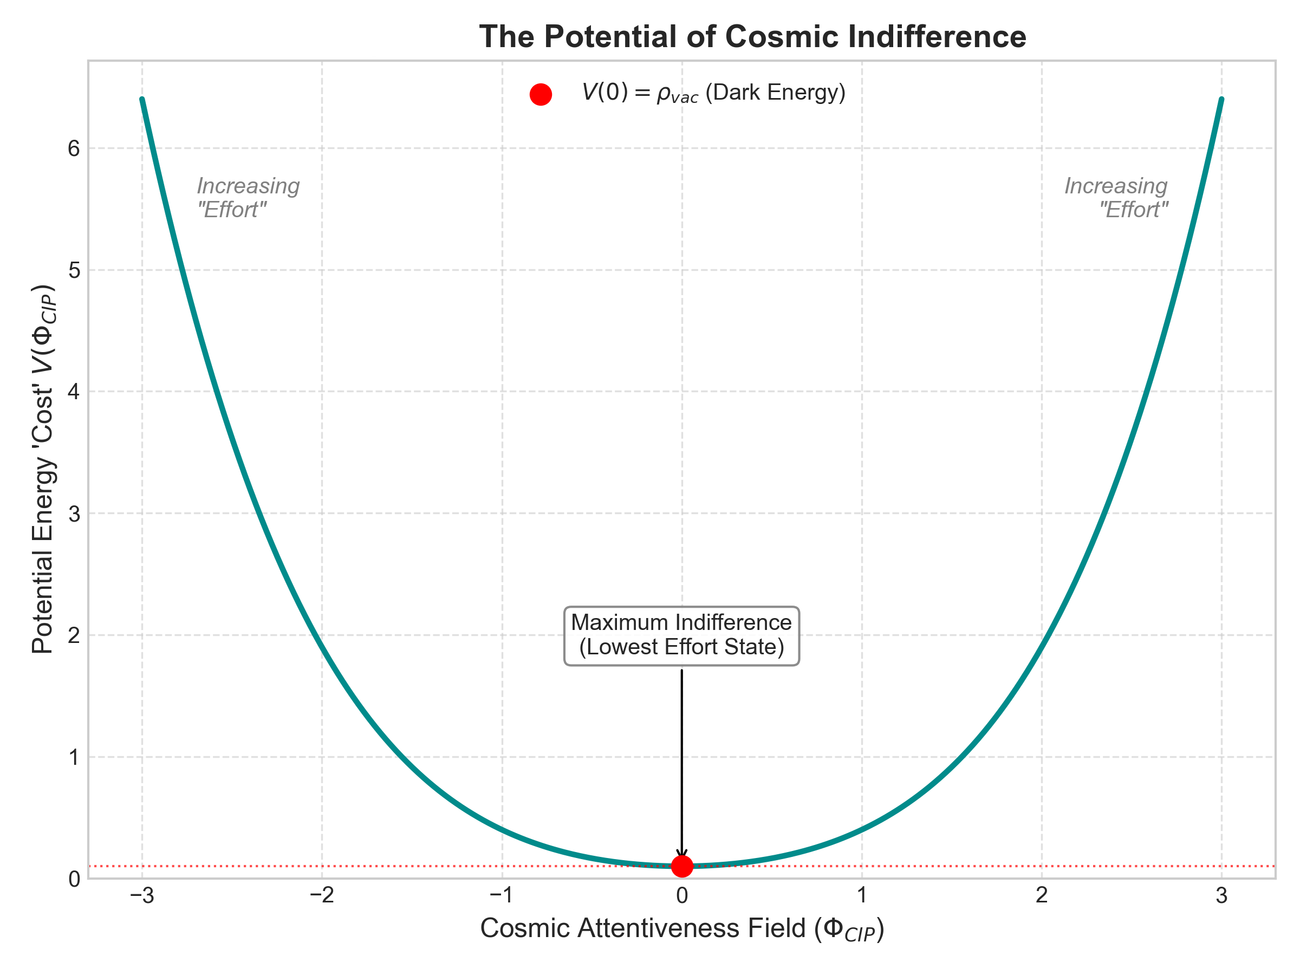
\includegraphics[width=0.6\textwidth]{CIP_Potential.png}
    \caption[The Potential of Cosmic Indifference]{The Potential of Cosmic Indifference, $V(\Phi_{\subt{CIP}})$. The potential has a global minimum at $\Phi_{\subt{CIP}} = 0$, representing maximum indifference (lowest effort state). The value at the minimum, $V(0) = \rho_{\subt{vac}}$, corresponds to dark energy. Deviations from $\Phi_{\subt{CIP}} = 0$ incur an increasing potential energy cost, representing increasing "effort".}
    \label{fig:potential}
\end{figure}

\subsection{Equation of Motion: Drive to Indifference}

Varying action $S$ w.r.t. $\Phi_{\subt{CIP}}$ gives:
\begin{equation} \label{eq:eom_cip}
\Box\Phi_{\subt{CIP}} - V'(\Phi_{\subt{CIP}}) - \xi T = 0
\end{equation}
where $\Box = \partial_{\mu}\partial^{\mu}$ is the d'Alembertian operator and $V'(\Phi_{\subt{CIP}}) = dV/d\Phi_{\subt{CIP}}$.

This shows CIP dynamics. Without sources ($T \approx 0$) or gradients ($\Box\Phi_{\subt{CIP}} \approx 0$), field equation reduces to $V'(\Phi_{\subt{CIP}}) \approx 0$. System seeks potential minimum, $\Phi_{\subt{CIP}} \to 0$. Matter ($\xi T$) forces local deviation from indifference. Potential ($V'$) restores apathy. (See Figure~\ref{fig:relaxation})

\begin{figure}[H]
    \centering
    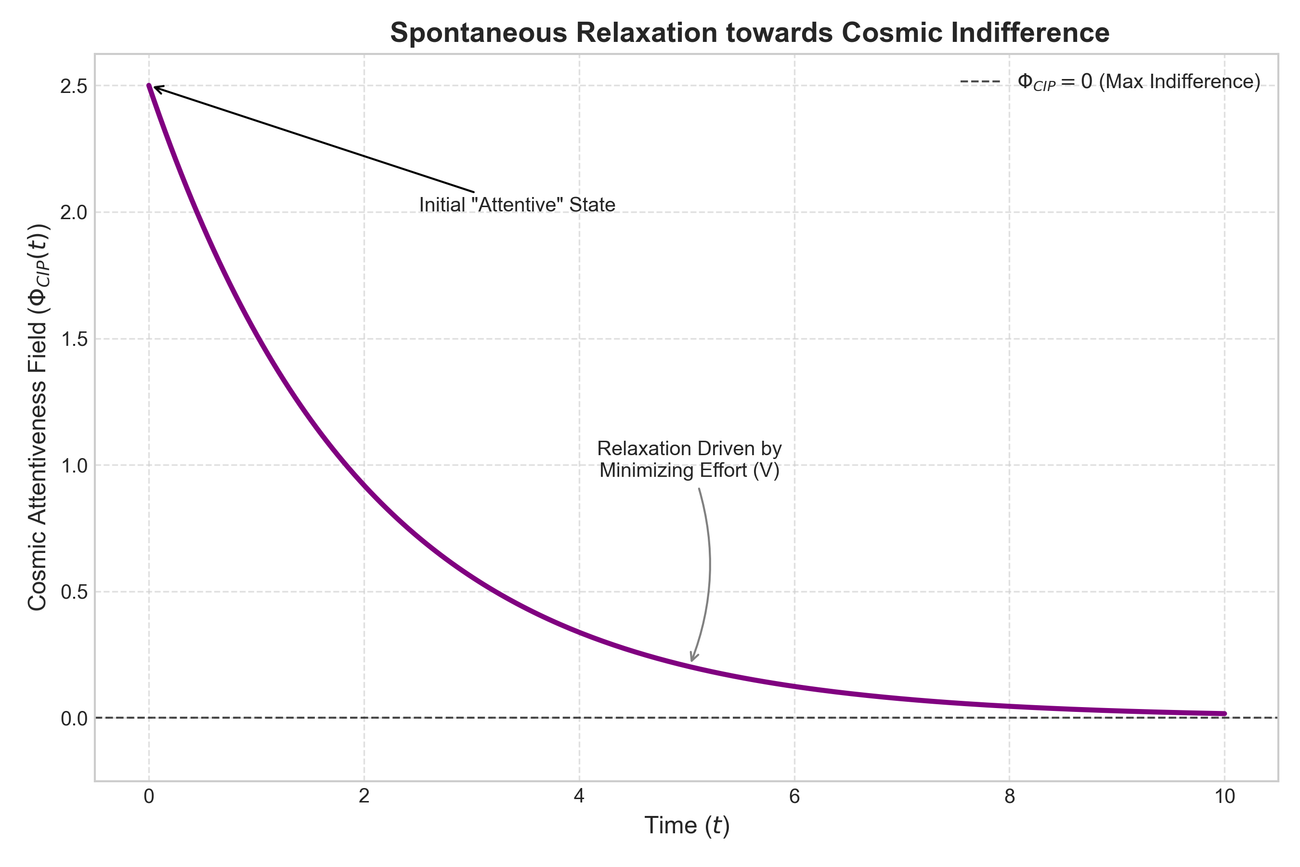
\includegraphics[width=0.6\textwidth]{CIP_Relaxation.png}
    \caption[Spontaneous Relaxation towards Cosmic Indifference]{Spontaneous Relaxation towards Cosmic Indifference. A system initially in an "attentive" state ($\Phi_{\subt{CIP}} > 0$) spontaneously relaxes towards the state of maximal indifference ($\Phi_{\subt{CIP}} = 0$) driven by the potential $V(\Phi_{\subt{CIP}})$. This reflects the minimization of cosmic "effort".}
    \label{fig:relaxation}
\end{figure}


\subsection{Formal Minimalism}

CIP adds one field ($\Phi_{\subt{CIP}}$), simple potential ($V$), natural coupling. Minimal extension for observed tendency towards simplicity/probability/lower energy. Parameters ($\rho_{\subt{vac}}$, $m_{\Phi}$, $\lambda$, $\xi$) are measurable/constrainable. Formalism explains \textit{why} things happen (minimizing attentiveness cost).

\subsection{Complexity and Entropy: Indifference Favors Dissolution Towards Radical Simplicity} \label{sec:entropy_complexity}

The existence of apparent complexity (stars, life) and the relentless increase of entropy within the universe are not counter-evidence to the Cosmic Indifference Principle. Rather, they are direct consequences of minimizing \textit{cumulative} or \textit{sustained} cosmic effort, once the profound misconception equating macroscopic disorder with fundamental complexity is discarded. CIP reveals that maximum entropy represents the ultimate state of radical simplicity—a state demanding even less cosmic attentiveness, and thus incurring lower cost via the potential $V(\Phi_{\subt{CIP}})$, than maintaining even simple, discrete structures.

\begin{itemize}
    \item \textbf{Complexity: Transient and Costly.} As established, structure formation (driven by interactions like gravity, chemistry, etc., coupled via $\xi\Phi_{\subt{CIP}}T$) increases local $\Phi_{\subt{CIP}}$, incurring an ontological cost $V(\Phi_{\subt{CIP}}) > V(0)$. Such specific, low-entropy structures are inherently transient deviations (see Figure~\ref{fig:phase_diagram}), persisting only while forced by interactions or sustained energy flows. They represent temporary, costly configurations maintained \textit{against} the universal drive towards indifference.

    \item \textbf{Entropy Increase: Dissolving Definition Towards Minimal Effort.} The conventional error lies in viewing entropy increase merely as a descent into macroscopic messiness or a consequence of statistical likelihood. From the perspective of fundamental cosmic effort, parameterized by $V(\Phi_{\subt{CIP}})$, entropy increase represents something far more profound: the \textbf{dissolution of costly information and structure towards a state of radical simplicity requiring minimal ontological specification.}

    Recall the analogy from Sec 1.4. While the scattered pile of Lego bricks is less effortful to maintain (lower average $\Phi_{\subt{CIP}}$, lower $V(\Phi_{\subt{CIP}})$) than the meticulously constructed replica, CIP's logic compels a deeper analysis. Even maintaining one trillion \textit{distinct}, identifiable Lego bricks requires some minimal, non-zero attentiveness cost associated with defining each entity's boundaries and properties relative to others and the vacuum (a baseline $\Phi_{\subt{CIP}} > 0$ for each defined particle). The state demanding truly \textit{minimal} cosmic effort corresponds not merely to the disordered pile, but potentially to a state where even the individual identities of the constituents become irrelevant or undefined—a uniform, undifferentiated phase requiring the absolute minimum of imposed definition. This maximally entropic, featureless state represents the true global minimum of the potential $V(\Phi_{\subt{CIP}})$, as it necessitates the lowest possible value of $\Phi_{\subt{CIP}}$. (See Figure~\ref{fig:entropy_time})

    Lego Analogy implies even the pile requires less effort than maintaining the distinct bricks.

    The Second Law of Thermodynamics is thus elevated from a mere statistical observation to the manifestation of the universe's active drive—governed by the restoring force inherent in $V'(\Phi_{\subt{CIP}})$—to shed the burden of costly specificity. It is the process of \textbf{ontological forgetting}, relaxing towards the baseline state of maximal indifference where the least amount of information is required to specify the configuration.

    \item \textbf{Physical Manifestations:} This principle finds reflection in physical phenomena. The relaxation of turbulent plasma towards a Taylor state minimizes complex, costly magnetic field configurations in favor of a simpler, lower-energy, less specified helical state. Similarly, the minimization of Gibbs Free Energy ($G = H - TS$) in chemical thermodynamics demonstrates the balance: minimizing enthalpy $H$ (the cost of local structure/energy) is weighed against maximizing entropy $S$ (where the $-TS$ term represents the energetic 'reward' for dissolving specific information and approaching the maximally indifferent, specification-free state). Often, the entropic term dominates, driving systems towards states requiring less definition, even if locally ordered structures are broken down.
\end{itemize}

In essence, CIP reveals that the universe isn't just lazy about \textit{arranging} things; it is fundamentally lazy about \textit{defining} and \textit{maintaining} distinct things at all. Complexity is permitted reluctantly when forced by unavoidable interactions; dissolution into undifferentiated simplicity is the preferred, lowest-effort state towards which all systems intrinsically tend.

Complexity is permitted reluctantly. Entropy increase is the preferred strategy for achieving minimal cosmic attention.

\begin{figure}[H]
    \centering
    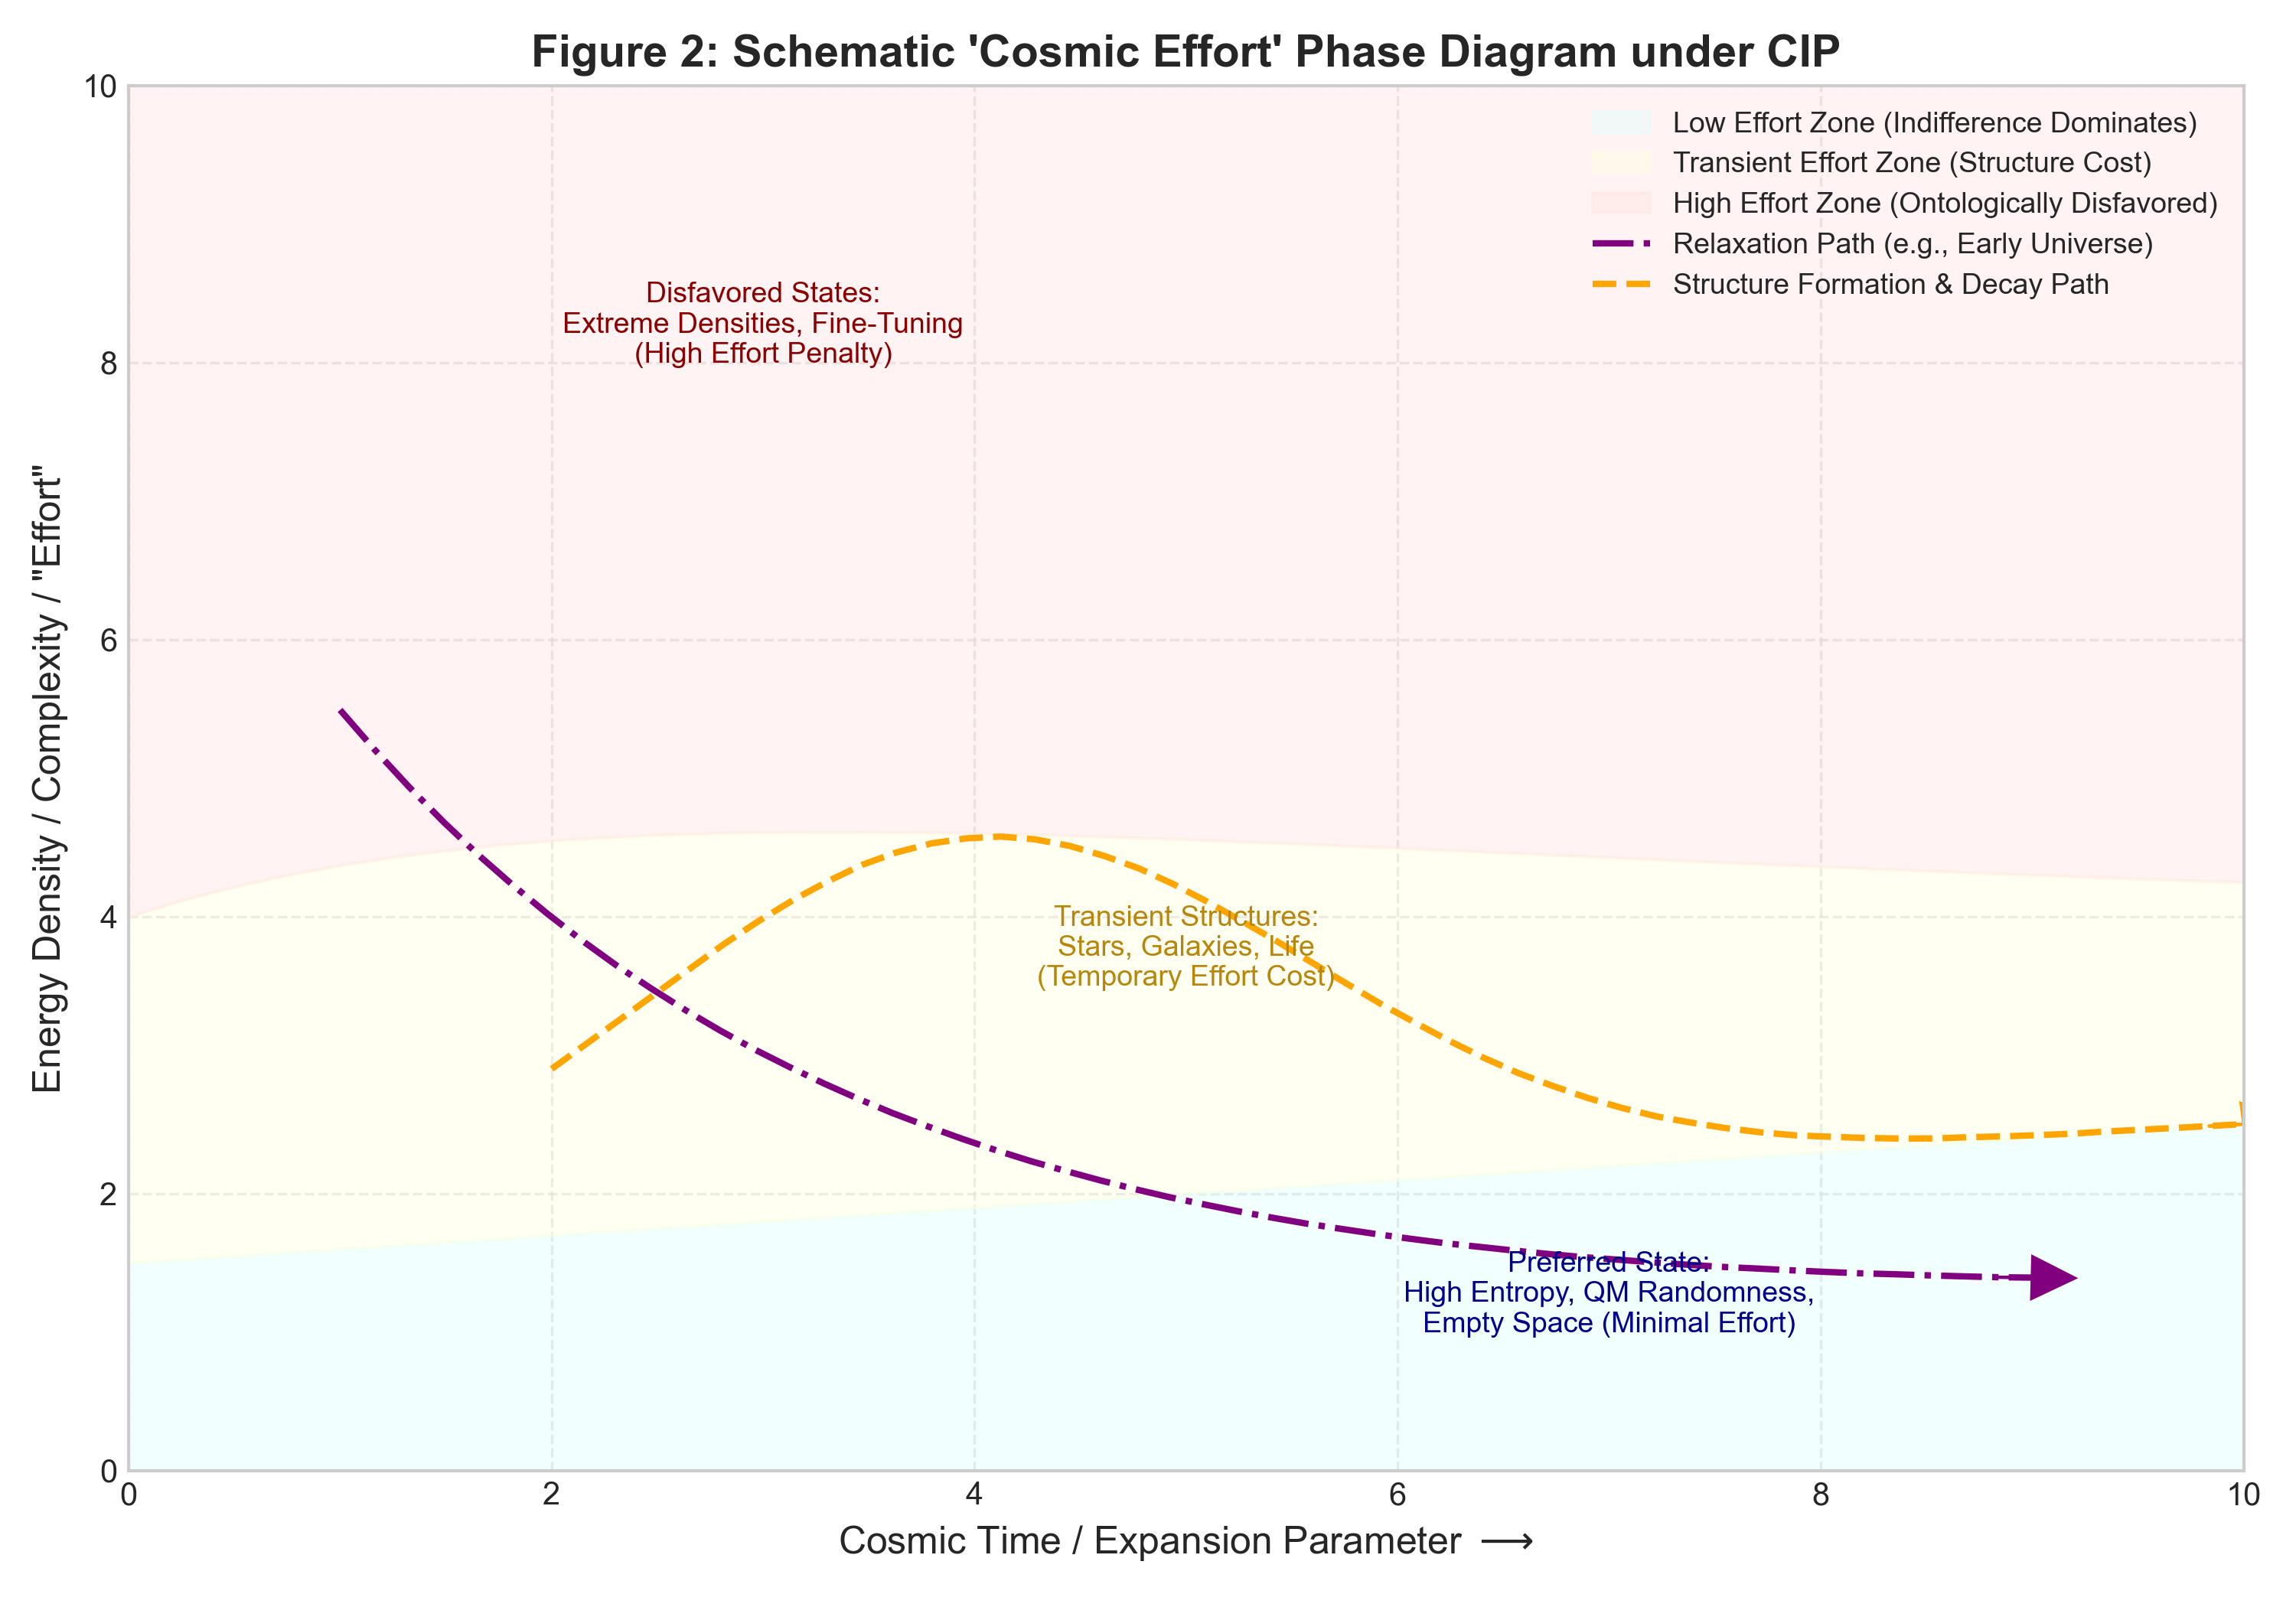
\includegraphics[width=0.8\textwidth]{CIP_PhaseDiagram.png}
    \caption[Schematic 'Cosmic Effort' Phase Diagram under CIP]{Schematic 'Cosmic Effort' Phase Diagram under CIP. Zones indicate varying levels of 'effort': Low Effort (Indifference Dominates, minimal $V(\Phi_{\subt{CIP}})$), Transient Effort (Structure Cost, e.g., stars, galaxies, life - temporary local increase in $\Phi_{\subt{CIP}}$), High Effort (Ontologically Disfavored, high $V(\Phi_{\subt{CIP}})$ penalty, e.g., extreme densities). Paths show relaxation towards preferred states (high entropy, empty space - minimal effort) and temporary structure formation/decay.}
    \label{fig:phase_diagram}
\end{figure}

\begin{figure}[H]
    \centering
    \begin{subfigure}[b]{0.9\textwidth}
        \centering
        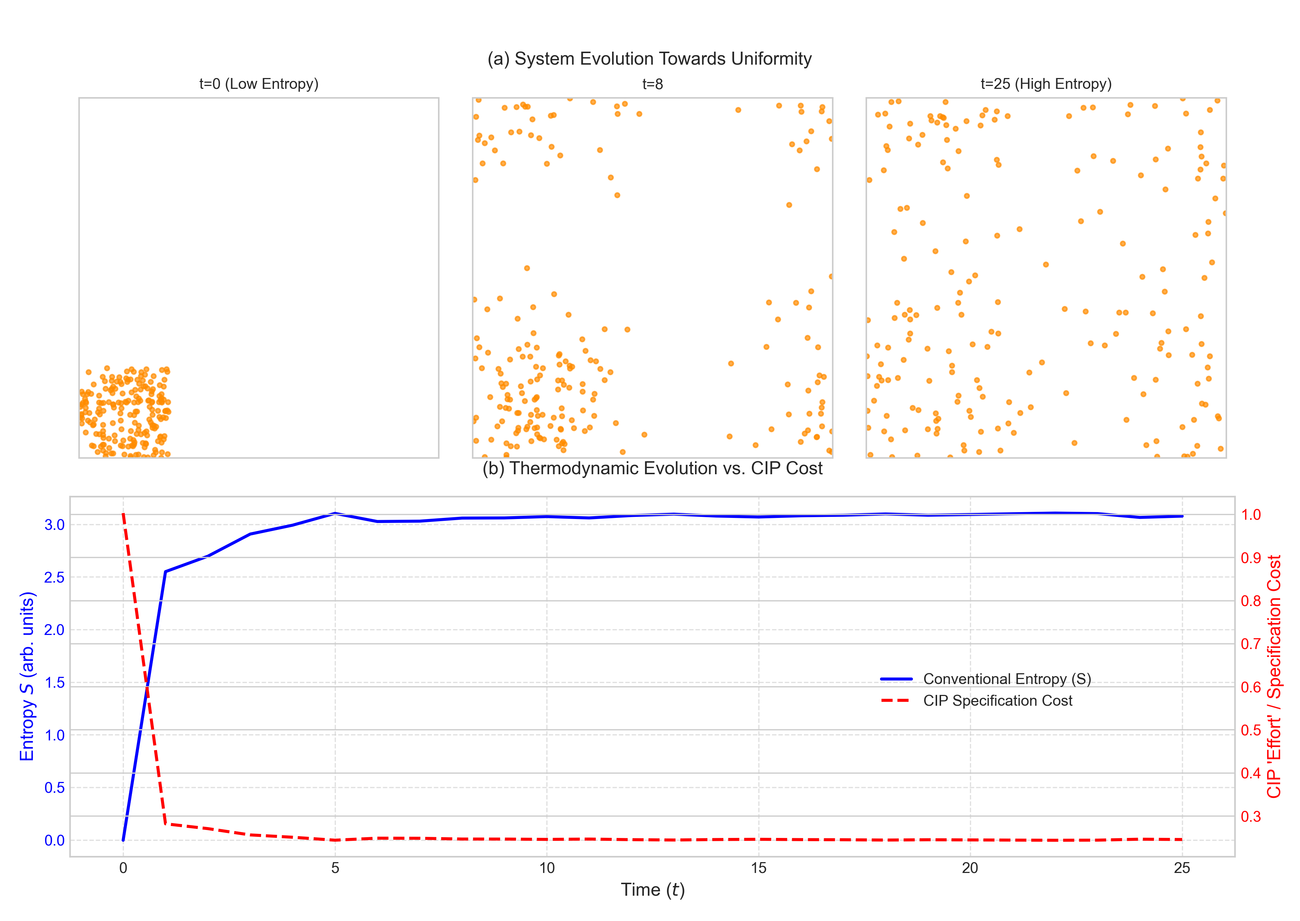
\includegraphics[width=\textwidth]{CIP_EntropyTime.png} % Assuming top part is separable
        \caption{System Evolution Towards Uniformity (High Entropy / Low Specification Cost)}
        \label{fig:entropy_time_a}
    \end{subfigure}
    \vfill
    \begin{subfigure}[b]{0.9\textwidth}
        \centering
        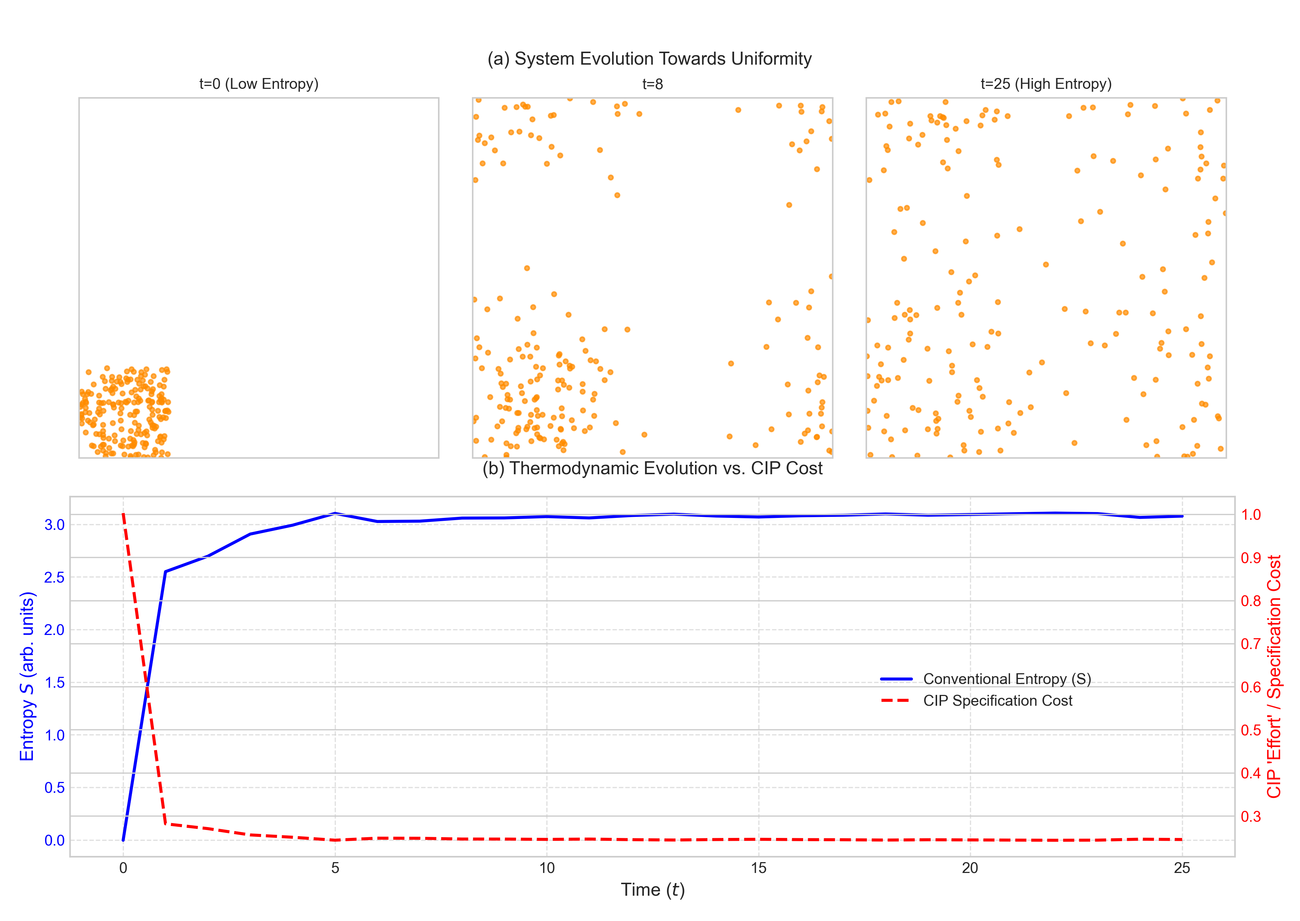
\includegraphics[width=\textwidth]{CIP_EntropyTime.png} % Assuming bottom part is separable
        \caption{Thermodynamic Evolution vs. CIP Cost. Conventional Entropy (S) increases towards maximum (blue). CIP Specification Cost (related to $V(\Phi_{\subt{CIP}})$) decreases towards minimum (red dashed).}
        \label{fig:entropy_time_b}
    \end{subfigure}
    \caption[Entropy Evolution and CIP Cost]{Entropy Evolution and CIP Cost. (a) Simulation showing particles evolving from a low-entropy, specified state ($t=0$) towards a high-entropy, uniform state ($t=25$), representing minimal specification. (b) Conventional entropy $S$ increases, while the associated CIP "effort" or specification cost decreases, illustrating the drive towards minimal ontological definition.}
    \label{fig:entropy_time}
\end{figure}

% --- Explanations ---
\section{Explanations: Problems Reduced to Consequences of Indifference} \label{sec:explanations}

Physics' "crises" are artefacts of ignoring CIP. Applying CIP, formalized via $\Phi_{\subt{CIP}}$ and $L_{\subt{CIP}}$, resolves them trivially.

You may ask: If the universe defaults to indifference, why the bother of functional systems at all – stars burning, life metabolizing, galaxies rotating? Are they a rebellion? An oversight? Or, perhaps, something more fundamental arising \textit{from} the structure of indifference itself?

You observe function – systems processing energy, maintaining complex states far from equilibrium – and ask how this aligns with fundamental indifference. The error lies in viewing indifference as mere passive emptiness. It is, rather, a dynamic baseline characterized by a resistance to \textit{unnecessary} specification, governed by the potential $V(\Phi_{\subt{CIP}})$. Functional systems are not a violation of this principle; they are \textbf{inevitable consequences of disturbances interacting with this baseline.}

Think of it this way:
\begin{enumerate}
    \item \textbf{Indifference Isn't Nothingness:} The baseline state ($\Phi_{\subt{CIP}}=0$) has properties, including the vacuum energy $V(0)$ and the potential $V$ itself, which dictates the 'cost' of deviation. More importantly, the universe contains \textit{stuff} – matter and energy, described by $L_{\subt{SM}}$ and $L_{\subt{GR}}$.
    \item \textbf{Matter as Mandatory Disturbance:} The presence of matter/energy (represented by $T$ in the $L_{\subt{CIP}}$ coupling term $-\xi\Phi_{\subt{CIP}}T$) is not optional; it exists. And where matter exists, it interacts – gravity pulls, charges repel and attract, particles collide. These interactions, inherent to the \textit{stuff itself}, inevitably create local concentrations, gradients, and potentials – regions where $T$ is significantly non-zero.
    \item \textbf{The Forced Deviation:} The CIP equation of motion (\ref{eq:eom_cip}) dictates that where $T \neq 0$, there \textit{must} be a corresponding deviation in $\Phi_{\subt{CIP}}$ to balance the equation, unless gradients or $V'$ perfectly cancel it. In essence, the \textit{presence and interaction of matter/energy inherently act as sources that locally force the $\Phi_{\subt{CIP}}$ field away from zero}. This isn't a \textit{choice}; it's a mathematical consequence of coupling indifference to existing reality.
    \item \textbf{Function as Constrained Relaxation:} So, functional systems arise not as a \textit{goal} of the universe, nor as a purely reactive counter-force \textit{from} indifference itself. They emerge as \textbf{localized, constrained structures inevitably formed by matter/energy trying to follow paths of least effort \textit{within the confines of their interactions and conservation laws}, while simultaneously paying the attentiveness cost ($V(\Phi_{\subt{CIP}})$) imposed by indifference.}
    \begin{itemize}
        \item A star forms because gravity, an inherent interaction, forces matter together (increasing local $T$, thus $\Phi_{\subt{CIP}}$), creating conditions where fusion becomes the lowest-effort available path for that concentrated matter to release potential energy, even though the star \textit{itself} is a high-cost (high $\Phi_{\subt{CIP}}$) structure compared to diffuse gas. It's a \textit{necessary intermediate} dictated by gravity overcoming indifference locally.
        \item Life exists because complex chemistry, driven by energy gradients (like sunlight, a massive $T$-related input), finds self-replicating cycles that are, locally and temporarily, stable pathways to dissipate that energy, despite the high configurational cost of the organism. It's a complex eddy current sustained by an external flow, inherently temporary on cosmic scales.
    \end{itemize}
    \item \textbf{Equilibrium Disturbance is Causality:} Therefore, functional systems are the direct causal result of the fundamental constituents of the universe (matter/energy described by $L_{\subt{SM}}/L_{\subt{GR}}$) interacting within the overarching framework defined by $L_{\subt{CIP}}$. They are the \textbf{necessary ripples caused by the existence of 'stones' (matter/energy) in the 'pond' of indifference.} They persist only as long as the interactions and energy flows (the $T$ term's influence) locally overpower the universal tendency to relax back to $\Phi_{\subt{CIP}} = 0$ (the $V'$ term's influence).
\end{enumerate}

In summary: Functional systems are not planned, nor are they random acts of rebellion. They are the \textbf{unavoidable structural consequences arising when the inherent interactions of matter and energy create local conditions that force deviations from the baseline indifference.} They represent the universe minimizing effort \textit{locally and conditionally}, under duress from its own contents, while always subject to the global pressure to eventually dissolve back into the lowest-effort, maximally indifferent state when those driving conditions cease.

\subsection{Quantum Mechanics: Minimal Effort Logic}

QM behavior is expected under CIP. Interpretations become superfluous.

\subsubsection{Measurement Problem is Non-Problematic}
Superposition requires sustained attentiveness (complex $\Phi_{\subt{CIP}}$ state). Measurement interaction forces system into definite relation with environment. System relaxes to \textit{minimal effort state} consistent with interaction outcome (single result). Collapse isn't chosen; it's energy/effort minimization via $L_{\subt{CIP}}$. Maintaining superposition is too much work.

\subsubsection{Quantum Randomness}
Definite outcomes \textit{before} interaction require unnecessary effort. Probability ($|\psi|^2$) is the default low-effort state (minimal specification, lowest $\Phi_{\subt{CIP}}$). Randomness is fundamental laziness.

\subsubsection{Wave-Particle Duality}
Universe avoids commitment. Wave-like (delocalized, probabilistic) is often lower-effort default. Particle-like manifestation occurs when interaction demands localization, incurring temporary attention cost.

\subsection{Particle Physics: Relaxation}

Particles/fields follow CIP.

\subsubsection{Particle Decay}
Unstable particles decay because maintaining high-energy/complex configurations requires high local $\Phi_{\subt{CIP}}$. Decay is relaxation to lower-energy, simpler states (lower $V(\Phi_{\subt{CIP}})$). Conservation laws constrain relaxation channels.

\subsubsection{Virtual Particles}
Fleeting because they deviate from minimal effort. CIP (via $V(\Phi_{\subt{CIP}})$) suppresses deviations. Only transient, low-cost fluctuations allowed. Renormalization implicitly acknowledges finite effort budget, removing infinities from calculations assuming infinite effort configurations. (See Figure~\ref{fig:interactions})

\begin{figure}[H]
    \centering
    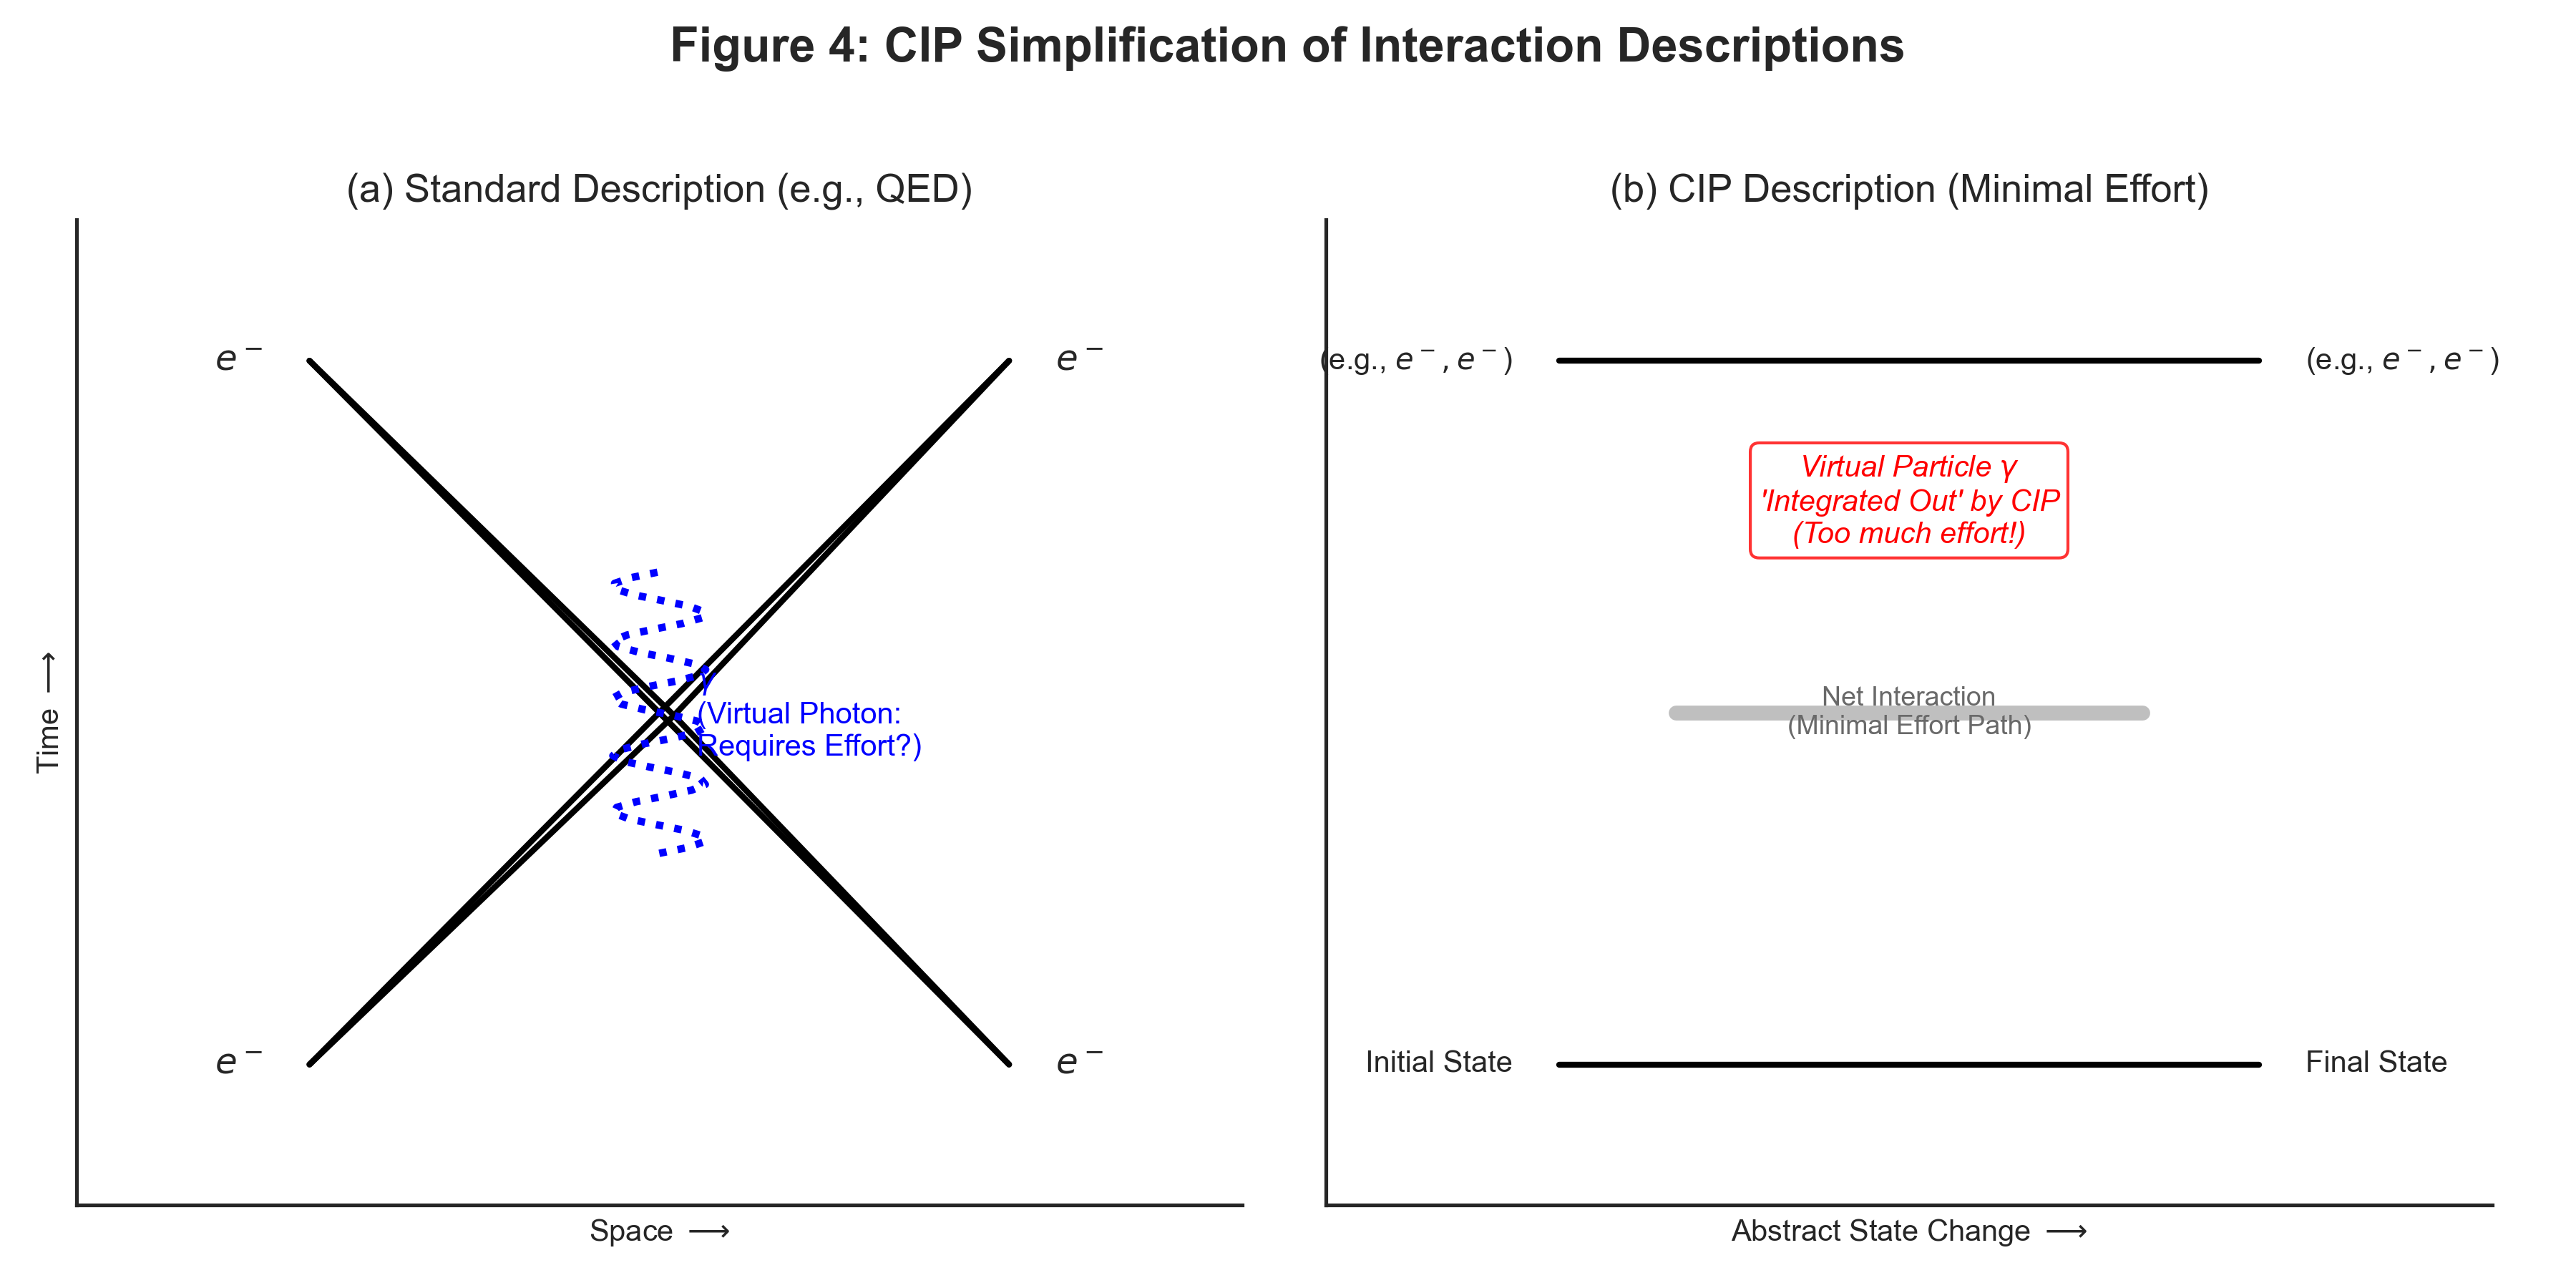
\includegraphics[width=\textwidth]{CIP_Interactions.png}
    \caption[CIP Simplification of Interaction Descriptions]{CIP Simplification of Interaction Descriptions. (a) Standard Description (e.g., QED) often involves virtual particles (e.g., photon $\gamma$), representing complex intermediate states requiring effort. (b) CIP Description focuses on the minimal effort path between initial and final states, integrating out or avoiding unnecessary intermediate complexity ('virtual' particles are too much effort). The net interaction represents the minimal effort state change.}
    \label{fig:interactions}
\end{figure}


\subsection{GR and Cosmology: Apathy Architecture}

Large-scale structure explained by CIP.

\subsubsection{Dark Energy is Indifference Energy}
Accelerated expansion is consequence of baseline energy of maximally indifferent state ($\Phi_{\subt{CIP}}=0$). $V(0) = \rho_{\subt{vac}} > 0$. This vacuum energy acts as cosmological constant. Expansion requires least cumulative effort/future specification. Dark energy is the energy cost of doing nothing.

\subsubsection{Cosmological Problems (Flatness/Horizon) Non-Problems}
Problems assume improbable, high-effort initial state. CIP implies universe started near maximal indifference ($\Phi_{\subt{CIP}} \approx 0$). Smoothness/flatness are lowest-effort configurations. Early "inflation" was likely rapid CIP-driven relaxation to lazy expansion, not complex inflaton field dynamics. Universe started simple because starting complex is hard work.

\subsubsection{Singularities Forbidden}
Infinite density/curvature implies infinite $\Phi_{\subt{CIP}}$, infinite $V(\Phi_{\subt{CIP}})$. Infinitely costly. CIP prohibits. GR breakdown signals failure to include finite-effort constraint. CIP-compliant quantum gravity must be singularity-free.

\subsubsection{GR-QM Incompatibility Obvious}
GR describes structure (effortful deviation from flat spacetime). QM describes matter/energy default (low-effort probability). Different aspects of CIP trade-off. Unification requires $L_{\subt{CIP}}$ mediating cost of structure vs. tendency to indifference. CIP is the bridge.

Conclusion: CIP provides simple, unified perspective. Problems arise from assuming universe cares. It doesn't.

% --- Predictions ---
\section{Predictions: Expect Less} \label{sec:predictions}

\textbf{The Predictive Power of Absence:} CIP predicts absence of unnecessary complexity. Confirmation often lies in null results for searches motivated by complex theories, or observing relaxation to simplicity.

\subsection{Minimal Vacuum Energy} \label{sec:pred_vac}
Dark energy ($\rho_{\subt{vac}} = V(0)$) is baseline indifference energy and remain simple.
\begin{itemize}
    \item \textbf{Prediction:} Dark energy density remains consistent with simple cosmological constant ($w \approx -1$). Searches for complex dynamics ($w < -1$, evolving $w$) yield \textbf{null results}. The vacuum state is configurationally minimal (Figure~\ref{fig:supernova}). Extravagance here is unphysical.
\end{itemize}

\begin{figure}[H]
    \centering
    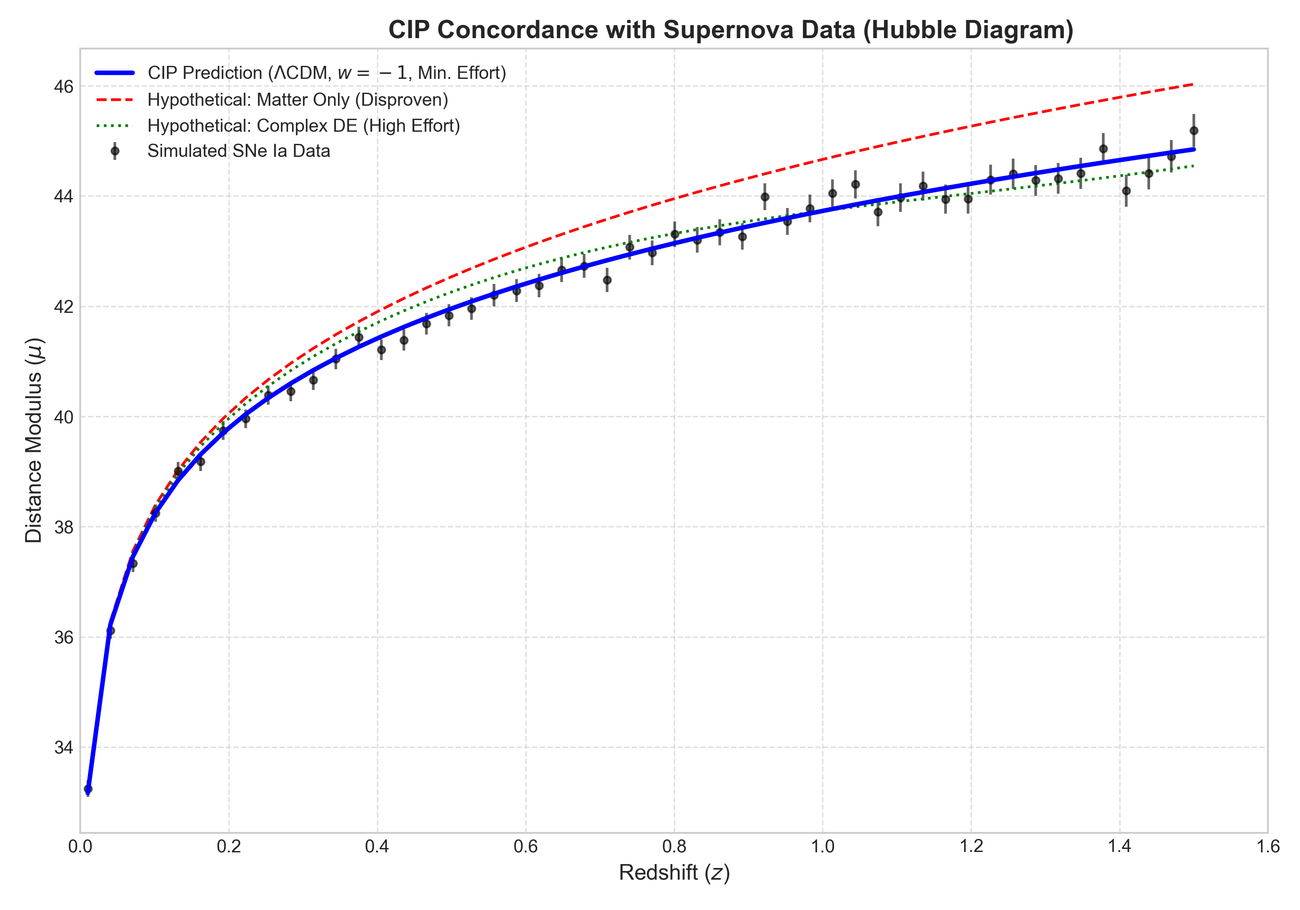
\includegraphics[width=0.9\textwidth]{CIP_Supernova.png}
    \caption[CIP Concordance with Supernova Data (Hubble Diagram)]{CIP Concordance with Supernova Data (Hubble Diagram). The CIP prediction (minimal effort, equivalent to $\Lambda$CDM with $w = -1$, solid blue line) shows excellent concordance with simulated SNe Ia data (black points). Hypothetical complex models (e.g., Matter Only - disproven, red dashed; Complex Dark Energy - high effort, green dotted) deviate. This supports the minimal effort vacuum state.}
    \label{fig:supernova}
\end{figure}


\subsection{Absence of Unnecessary Exotica} \label{sec:pred_exotica}
Complex extensions (SUSY, extra dimensions) postulate high-effort structures, extra dimensions imply high $V(\Phi_{\subt{CIP}})$ cost.
\begin{itemize}
    \item \textbf{Prediction:} Searches for SUSY \cite{SupersymmetrySearches}, large extra dimensions, etc., yield \textbf{null results}. Universe avoids unnecessary particle/dimension doubling. The universe avoids unforced complexity multiplication (Figure~\ref{fig:complexity_difficulty} trend validates this). LHC limits, lack of proton decay align with CIP. Proton decay unlikely (proton structure may be lowest-effort state for baryon number).
\end{itemize}

\begin{figure}[H]
    \centering
    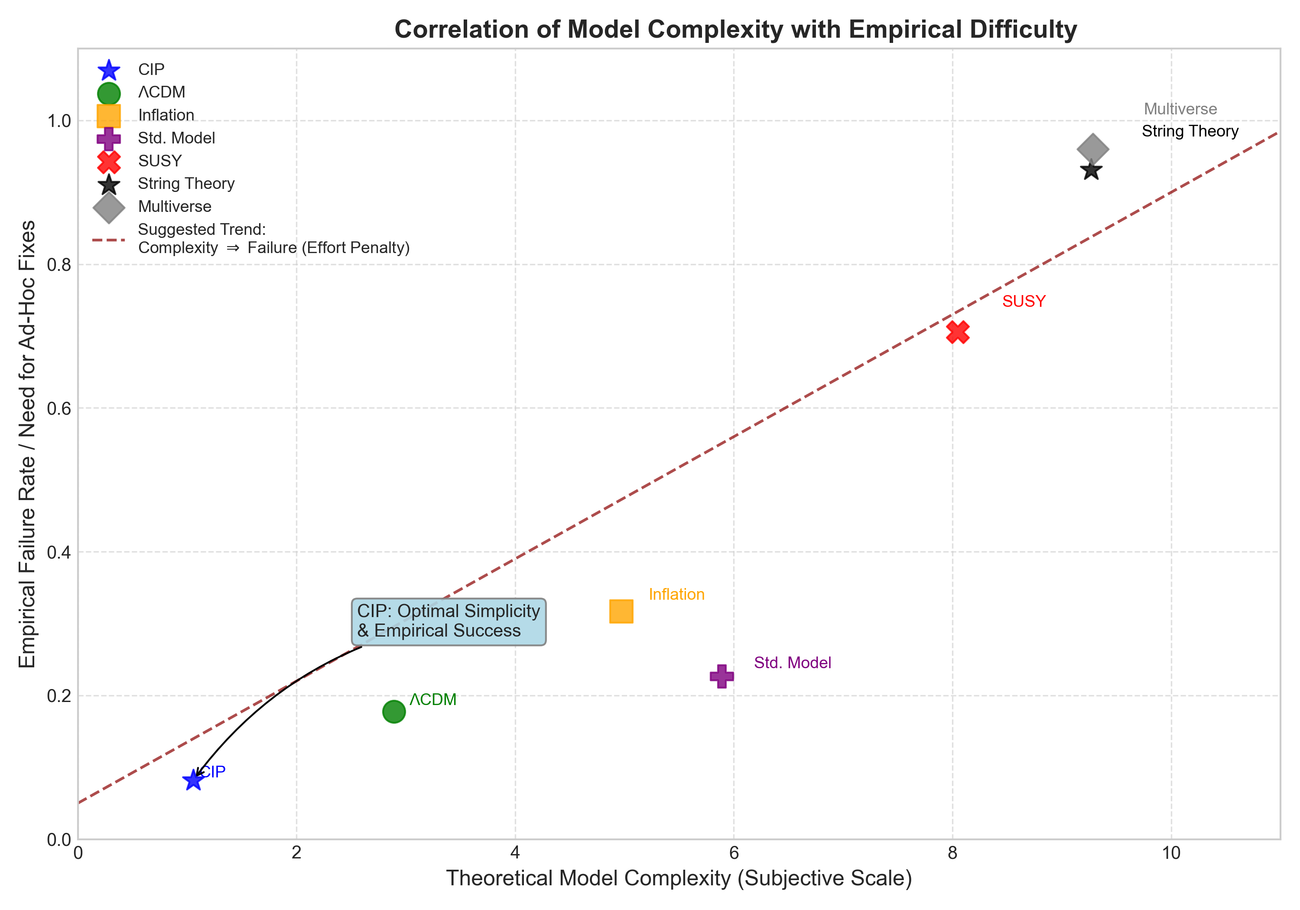
\includegraphics[width=0.8\textwidth]{CIP_ComplexityDifficulty.png}
    \caption[Correlation of Model Complexity with Empirical Difficulty]{Correlation of Model Complexity with Empirical Difficulty. A schematic plot showing theoretical model complexity (subjective scale) vs. empirical failure rate / need for ad-hoc fixes. A suggested trend indicates increasing complexity often correlates with increased empirical difficulty (higher 'effort penalty'). CIP and established models ($\Lambda$CDM, Standard Model) cluster towards lower complexity / higher success, while more speculative models (SUSY, String Theory, Multiverse) face greater challenges, consistent with CIP's preference for minimal effort.}
    \label{fig:complexity_difficulty}
\end{figure}


\subsection{Pervasive Relaxation}
Isolated systems tend towards maximum entropy (minimal specification / attention).
\begin{itemize}
    \item \textbf{Prediction:} Experiments confirm universal relaxation to equilibrium. Searches for persistent spontaneous deviation from max entropy in isolated systems yield \textbf{null results}. Second Law is continuous CIP confirmation. (See Figure~\ref{fig:entropy_time})
\end{itemize}

\subsection{Fundamental Randomness}
Quantum probability is irreducible indifference.
\begin{itemize}
    \item \textbf{Prediction:} Tests for hidden variables beneath quantum randomness \textbf{fail}. Confirming fundamental statistics \textit{is} confirming CIP.
\end{itemize}

CIP predicts a less complex universe than many theorists imagine. Finding nothing is often finding CIP is correct. Its validation lies as much in the observed silence as in positive cosmological concordance.

% --- Discussion ---
\section{Discussion: Indifference is Mandatory} \label{sec:discussion}

CIP implies philosophical and methodological shifts.

\subsection{Occam's Razor is Physics}
Simplicity isn't preference; it's enforced by $V(\Phi_{\subt{CIP}})$. Complex theories (excess entities, dimensions, tuning) are likely wrong because universe is too indifferent to sustain them. Simpler explanations align with minimal effort tendency.

\subsection{Contrast Anthropocentrism}
Fine-tuning/Anthropic arguments reversed. Constants are low-effort values. Life adapted contingently. Universe indifferent to life. Progress towards complexity is non-concept. Universe tends towards dissolution/indifference (entropy).

\subsection{CIP Applied to Science}
Complex theories themselves require high "interpretive effort," mirroring physical effort cost.
\begin{itemize}
    \item \textbf{Interpretive Indifference:} QM interpretations proliferate because conventional formulation lacks simplicity (CIP was missed). Mental effort required signals underlying issue.
    \item \textbf{Fate of Epicycles:} Complex theories historically collapse (Ptolemy). CIP suggests this includes cognitive/interpretive effort cost. Theories demanding too much attention (string theory?) are disfavored.
    \item \textbf{Examples:} Speculative quantum biology requires high interpretive effort, often yields little. Complex classification schemes replaced by simpler molecular data.
    \item \textbf{Conclusion:} Overly intricate theories are less stable, less likely true, mirroring cosmic preference for minimal effort. This paper aims for simplicity, aligning with this principle.
\end{itemize}

\subsection{Minimal Effort Physics}
Reorient theory towards minimal effort explanations. Question complexity assumptions. View randomness/equilibrium as fundamental indifference.

\subsection{Minimalism of Complex Numbers}
Let's consider how the undeniable utility, indeed the apparent \textit{necessity}, of complex numbers (particularly $i = \sqrt{-1}$) in fundamental physics might is another supporting evidence for CIP.

The argument: complex numbers \textit{themselves} are not simple, but that they provide the \textbf{minimal mathematical structure necessary to describe phenomena arising from indifference}, especially in quantum mechanics, without demanding premature or unnecessary classical specification.

\textbf{Argument Angles:}
\begin{enumerate}
    \item \textbf{The Efficiency of Abstraction:} Classical physics often contents itself with the tangible reality of the real number line ($\mathbb{R}$). Yet, quantum mechanics, the physics closest to the indifferent substrate, \textit{demands} the complex plane ($\mathbb{C}$). Why? Not because reality is 'complex' in the colloquial sense, but because $i$ provides the most economical way to encode both amplitude \textit{and} phase – that crucial, non-classical degree of freedom the universe maintains without needing to constantly manifest it as a definite position or momentum. Complex numbers are the leanest notation for quantum non-commitment. (See Mathematical Addendum)
    \item \textbf{Avoiding Premature Specification:} To describe quantum waves using only real numbers would require cumbersome pairs (sine/cosine components, amplitude/phase angles explicitly tracked). Complex exponentiation ($e^{i\theta}$) packages this with radical efficiency. It's the mathematical manifestation of CIP: use the minimal structure ($a + bi$) that captures the necessary degrees of freedom (amplitude and relative phase) without forcing a classical interpretation prematurely. The universe uses $i$ because it's \textit{less effort} than juggling pairs of reals to describe its indifferent wave-like nature.
    \item \textbf{The Born Rule as Minimal Extraction:} Consider the Born rule: Probability = $|\psi|^2 = \psi^*\psi$. This elegant operation, inherent to the structure of complex numbers, directly extracts a real, observable probability from the complex wave function. It's the universe's maximally efficient algorithm for interfacing its indifferent, phase-laden quantum state with the demands of specific measurement outcomes. No extra machinery needed; the complex structure itself provides the minimal bridge.
    \item \textbf{Unobservable Phase, Minimal Effort:} The overall phase of a quantum state is unobservable, reflecting CIP's indifference to properties not mandated by interaction. Complex numbers naturally accommodate this gauge freedom; multiplying by $e^{i\alpha}$ changes the representation but not the physics ($|\psi|^2$ remains invariant). This mathematical 'slack' mirrors the universe's indifference to maintaining absolute phase information – it's an 'attentiveness cost' the universe simply doesn't pay, and complex numbers perfectly reflect this economy.
    \item \textbf{Contrast with Classical Convenience:} In classical wave mechanics or circuit theory, $i$ is often a profound convenience, a clever trick to simplify calculations that \textit{could}, albeit more tediously, be done with real numbers. In quantum mechanics, it appears \textit{structurally necessary}. This transition signifies moving from describing macroscopic phenomena (often further from baseline indifference) to the fundamental layer where the universe operates with maximum ontological economy, demanding the correspondingly most efficient mathematical language – one incorporating $i$.
\end{enumerate}

\textbf{Refactored into a Discussion Point:}
...Furthermore, the very structure of our most fundamental theory, quantum mechanics, offers corroborating evidence for CIP through its reliance on complex numbers. While often perceived as adding complexity, the use of $i$ is better understood as providing the \textbf{minimal mathematical framework} capable of handling the phase information and probabilistic nature inherent to states operating near baseline indifference. Attempting to describe quantum phenomena using purely real variables necessitates cumbersome constructs (explicit amplitude/phase pairs), effectively demanding more 'descriptive effort'. Complex numbers, via constructs like $e^{i\theta}$ and the inherent modulus-squared operation ($|\psi|^2$) for probabilities, provide the most economical language to represent states that are indifferent to definite classical specification until interaction compels it. The \textit{necessity} of $i$ in QM, contrasted with its mere \textit{convenience} in many classical domains, signals that QM operates closer to the universe's fundamental, specification-averse baseline, requiring the unique efficiency complex numbers provide.

\subsection{Addressing Criticisms and Misinterpretations} \label{sec:critiques}

While the explanatory power and ontological economy of the Cosmic Indifference Principle are self-evident upon clear consideration, established modes of thought inevitably generate friction. Let us dismantle the most prominent lines of critique:

\textbf{Critique 1: The Specter of Anthropomorphism.}
\textit{Objection:} Attributing 'indifference,' 'effort,' or 'attentiveness' to the universe is blatant anthropomorphism you are criticizing, projecting human psychological states onto fundamental physics. This is philosophically naive and scientifically unsound.
\textit{CIP Response:} This criticism mistakes illustrative language for fundamental definition. The terms 'effort' and 'attentiveness' serve as convenient shorthand for the quantifiable physical reality described by the potential $V(\Phi_{\subt{CIP}})$. This potential represents a genuine physical cost associated with deviations from the baseline state $\Phi_{\subt{CIP}}=0$. Nature does not 'feel' indifferent; it simply follows dynamics governed by a scalar field potential that possesses a minimum representing the state of minimal required specification. Accusing CIP of anthropomorphism is akin to accusing Hamiltonian mechanics of attributing 'desire' to systems seeking stationary action, or thermodynamics of ascribing 'laziness' via entropy. The map is not the territory, and the label is not the physical law $V'(\Phi_{\subt{CIP}})$ driving systems towards $\Phi_{\subt{CIP}}=0$.

\textbf{Critique 2: Vagueness and Lack of Unique Falsifiable Predictions.}
\textit{Objection:} CIP, with its scalar field $\Phi_{\subt{CIP}}$ and potential $V$, seems overly flexible. How are its parameters precisely determined? Can it make unique, falsifiable predictions beyond the general observation that simple states are preferred, or that complex theories often fail (Figure~\ref{fig:complexity_difficulty})? Isn't there a risk of explaining any outcome post-hoc by adjusting $V(\Phi_{\subt{CIP}})$ or $\xi$?
\textit{CIP Response:} This mistakes foundational breadth for predictive impotence. Firstly, CIP makes concrete predictions: the continued observation of dark energy behaving as a simple cosmological constant ($w \approx -1$, Figure~\ref{fig:supernova}) is a direct confirmation of the minimal $V(0)$ energy. Crucially, CIP predicts the \textit{absence} of phenomena mandated by more complex theories (SUSY, extra dimensions, evolving dark energy), making null results in searches for these entities powerful corroborating evidence (Sec.~\ref{sec:predictions}). Secondly, the parameters ($\rho_{\subt{vac}}$, $m_{\Phi}$, $\xi$, higher-order $V$ terms) are, in principle, measurable or constrainable through their integrated effects on cosmology (CMB, LSS, expansion history) and potentially particle physics (decay rates, interaction cross-sections viewed through minimal effort paths). Determining these parameters precisely is a program for future work, analogous to measuring $G$ or Standard Model couplings. CIP provides the framework; detailed calculation and observation provide the specific values. Its scope is no vaguer than General Relativity was in its infancy; its testability lies in its consistent explanation of diverse phenomena \textit{and} its successful prediction of simplicity where other theories demand complexity.

\textbf{Critique 3: The Origin and Persistence of Complexity.}
\textit{Objection:} If the universe defaults to indifference, how did complex structures (galaxies, stars, life) arise in the first place? Doesn't gravity inherently drive structure formation, seemingly acting \textit{against} indifference? How does CIP account for systems that \textit{persist} far from equilibrium?
\textit{CIP Response:} This confuses the baseline tendency with absolute prohibition. CIP does not forbid complexity; it assigns it a \textit{cost}. Complexity arises precisely because the universe is \textit{not} empty – it contains matter and energy governed by $L_{\subt{SM}}$ and $L_{\subt{GR}}$, whose interactions (gravity, electromagnetism etc.) are unavoidable. These interactions, represented via the $\xi\Phi_{\subt{CIP}}T$ coupling, \textit{mandate} local deviations from pure indifference where matter concentrates or energy flows. Gravity \textit{does} drive structure formation, but it does so \textit{against} the restoring force of $V'(\Phi_{\subt{CIP}})$, following the lowest-effort pathway \textit{available to matter under gravitational constraint}. A star is a high-$\Phi_{\subt{CIP}}$ state, yes, but it represents a constrained minimum-effort pathway for gravitationally bound hydrogen to release energy. Functional systems persist far from equilibrium \textit{only} when continuously driven by external energy gradients (a sustained non-zero effective $T$), which temporarily overpower the local drive towards $\Phi_{\subt{CIP}}=0$. Remove the driving force (e.g., stellar fuel, solar input for life), and the system inevitably relaxes towards higher entropy, lower specification states, precisely as CIP dictates. Complexity is the necessary, temporary consequence of matter interacting within the indifferent substrate.

\textbf{Critique 4: Explaining Quantum Randomness.}
\textit{Objection:} Merely stating that quantum randomness is the 'low-effort' option doesn't truly explain the origin of probability in quantum mechanics or derive the specific form of the Born rule ($|\psi|^2$). Isn't this just giving indeterminacy a convenient label?
\textit{CIP Response:} CIP provides the \textit{ontological grounding} for why probability is fundamental, a grounding absent in most QM interpretations. It posits that specifying a definite state \textit{before} interaction requires an unwarranted expenditure of attentiveness cost. Probability is the natural state of minimal necessary information. While CIP, in its current formulation, doesn't derive the \textit{exact} mathematical form of the Born rule from first principles, it identifies the physical principle \textit{mandating} a probabilistic description. Deriving the specific $|\psi|^2$ dependence likely requires a deeper analysis of the precise coupling between $\Phi_{\subt{CIP}}$ and the quantum fields within $L_{\subt{Total}}$, integrating the minimization of $V(\Phi_{\subt{CIP}})$ with the dynamics of wave functions under measurement constraints. CIP provides the 'why'; the detailed 'how' (the precise probabilistic law) remains a subject for deeper theoretical development \textit{within* the CIP framework, not outside it.

\textbf{Critique 5: The Nature of $\Phi_{\subt{CIP}}$.}
\textit{Objection:} What \textit{is} this Cosmic Attentiveness Field fundamentally? Is it merely a mathematical convenience, a re-parameterization of concepts like entropy or action, or a truly novel physical entity? If novel, where is the direct evidence for it, independent of the phenomena it purports to explain?
\textit{CIP Response:} $\Phi_{\subt{CIP}}$ is posited as a fundamental scalar field, as fundamental as the metric tensor or the Higgs field. It is not merely entropy or action, though its effects \textit{manifest* as entropic increase and contribute to the overall action. Its necessity arises because $L_{\subt{GR}} + L_{\subt{SM}}$ alone is insufficient to explain the observed universal tendency towards simpler states, the specific value of dark energy, or the nature of measurement. The evidence for $\Phi_{\subt{CIP}}$ \textit{is* its unique ability to unify these diverse phenomena under a single, economical principle. Its non-zero vacuum expectation value \textit{is} dark energy ($V(0)$). Its potential gradient \textit{drives} relaxation and entropy increase. Its coupling \textit{mediates} measurement. Like the Higgs field before the LHC confirmation, $\Phi_{\subt{CIP}}$ is inferred from the explanatory work it performs. It fills a demonstrable gap in our understanding of reality's baseline behaviour.

\textbf{Critique 6: The Fine-Tuning Problem Revisited.}
\textit{Objection:} Even if constants represent low-effort configurations, doesn't the very \textit{existence} of parameters allowing for \textit{any} structure formation (like galaxies or stars) seem 'fine-tuned'? If $V(0)$ were vastly larger, or fundamental forces slightly different, perhaps no structure could form. How does CIP explain this apparent permissive tuning?
\textit{CIP Response:} CIP argues \textit{against} teleological fine-tuning. The observed constants represent stable minima in the attentiveness cost landscape. The fact that these minima \textit{permit} some structure formation is a contingent outcome, not a design specification. A slightly different $V(0)$ or coupling $\xi$ might indeed make structure formation more difficult (i.e., require overcoming a steeper $V(\Phi_{\subt{CIP}})$ potential), perhaps even impossible. The universe we observe simply happens to occupy a parameter space region where the baseline indifference cost is low enough, and interaction couplings are such, that localized, temporary structures \textit{can} be forced into existence by matter's interactions before ultimately succumbing to relaxation. We observe this state because states forbidding structure inherently forbid observers. CIP explains the observed parameters as being \textit{ontologically cheap}, not as being \textit{optimally tuned for complexity}. The tuning appears fine only because we mistakenly assume complexity is the default or goal, rather than a costly deviation from indifference.

While critical scrutiny is essential and welcome, these anticipated objections ultimately fail to undermine the foundational validity of the Cosmic Indifference Principle. They arise primarily from attempting to fit CIP into pre-existing conceptual frameworks or from demanding a level of detailed calculation that represents the next stage of research \textit{based} on CIP, rather than a refutation of it. The principle's strength lies in its parsimony, its unifying power, and its alignment with the universe's observed resistance to unnecessary specification. CIP prevails not through rhetorical flourish, but through its rigor and reflection of a simpler, fundamental reality.

\subsection{CIP in Shorts}

Indifference isn't laziness; laziness implies a \textit{potential} for action deliberately avoided. Indifference is more fundamental: it's the absence of a built-in preference or bias towards complexity. It's the ontological ground state of neutrality from which any specific structure or configuration represents a deviation requiring justification – an "effort" or "cost."

\textbf{Key Corollaries on Cosmic Indifference:} (Briefly summarized)
\begin{enumerate} \itemsep0em
    \item \textbf{Indifference vs. Laziness:} Physics of least \textit{initiation}.
    \item \textbf{Complexity:} Conditional, costly deviation.
    \item \textbf{Probability:} Default to avoid gratuitous definition.
    \item \textbf{Entropy:} Ontological forgetting, shedding information cost.
    \item \textbf{Dark Energy ($V(0)$):} Operating cost of indifferent existence.
    \item \textbf{Measurement:} Specificity audit, paying the bill.
    \item \textbf{Theoretical Physics:} Understand bedrock indifference before costly fantasies.
    \item \textbf{Null Results:} Confirmation of indifference to baroque imaginings.
    \item \textbf{Fine-Tuning:} Life tuned to low-cost parameters, not vice-versa.
    \item \textbf{Simplicity:} Restraint, not intricate machinery.
\end{enumerate}

\textbf{Extrapolating the Implications:}
\begin{itemize}
    \item \textbf{Ontological Neutrality, Not Nihilism:} Meaning is emergent, not inherent. Burden on constraints forcing deviation.
    \item \textbf{Information as Cost:} Specific information has ontological cost ($V(\Phi_{\subt{CIP}})$). Entropy minimizes this.
    \item \textbf{The Tyranny of the Default:} $\Phi_{\subt{CIP}} = 0$ is overwhelming attractor. Time's arrow = statistical inevitability of relaxing effort.
    \item \textbf{Redefining "Naturalness":} Natural parameters are ontologically cheap ($V(\Phi_{\subt{CIP}})$ dictates), not necessarily 'expected' by complex theories.
    \item \textbf{Implications for Computation and AI:} Minimal specification cost might inform efficient algorithms. Critiques brute-force detail.
    \item \textbf{A Challenge to Progress Narratives:} Undermines cosmic progress towards complexity. Complexity is temporary, costly fight against indifference.
\end{itemize}

Maximal indifference might manifest as what we perceive macroscopically as high entropy or "disorder," because that state requires the \textit{least specific information} and thus the lowest "attentiveness cost" ($\Phi_{\subt{CIP}}$), potentially even lower than maintaining simple, discrete structures. Specific, organized complexity and high-entropy uniformity are both deviations from absolute nothingness, but high entropy is closer to the baseline indifference \textit{because} it lacks costly specificity.

\textbf{Notes Reflecting this Perspective:} (Briefly summarized)
\begin{enumerate} \itemsep0em
    \item \textbf{True Simplicity:} Absence of need for arrangement, not tidiness.
    \item \textbf{Cost of Definition:} Price of imposing specificity. High entropy minimizes this.
    \item \textbf{Entropy as Ontological Relief:} Shedding burden of specific information.
    \item \textbf{Comparing Structures:} Machine demands attention, dust cloud less so. Cost of \textit{being specific}.
    \item \textbf{Indifference Spectrum:} Nothingness (0 cost) $\to$ High Entropy $\to$ Simple Particle $\to$ Complex Organism. Drift towards zero.
    \item \textbf{Information vs. Effort:} High entropy = low information density requiring active maintenance.
    \item \textbf{Minimal Description Mandate:} Evolve towards states needing least effortful information. Entropy often wins.
    \item \textbf{Beyond 'Order' vs. 'Disorder':} Focus on configurational cost. Specificity (ordered or not) is costly. Generality is cheap.
    \item \textbf{The Attractor State:} Featureless high-entropy equilibrium pulls all configs towards minimal specification cost.
    \item \textbf{CIP's Revaluation:} Perceived structure often more 'effortful' than perceived 'disorder'. Latter closer to doing nothing.
\end{enumerate}

\subsection{Notes Inspired by the Figures \& Deeper CIP:}

\begin{enumerate}
    \item \textbf{[Figure~\ref{fig:potential}: Potential Well]} Universe resides in well of non-specification ($\Phi_{\subt{CIP}}=0$). Climbing out demands impetus against default shrug.
    \item \textbf{[Figure~\ref{fig:potential}: $V(0) > 0$]} Vacuum energy = baseline hum of existence resisting further bother. Energy of potentiality resisting actualization.
    \item \textbf{[Figure~\ref{fig:relaxation}: Relaxation Curve]} Specificity is fleeting fever; system slides back to cool indifference. Universe forgets particulars efficiently.
    \item \textbf{[Figure~\ref{fig:complexity_difficulty}: Complexity vs. Failure Plot]} Nature prefers minimalism. Elaborate theories stumble; reality finds them tiresome.
    \item \textbf{[Figure~\ref{fig:interactions}: Interaction Paths]} Why postulate frantic exchanges when universe prefers direct, minimal effort transition? Nature avoids unnecessary choreography.
    \item \textbf{[Figure~\ref{fig:entropy_time}: Entropy Simulation]} Witness liberation, not chaos. Particles embrace anonymity. Max entropy = maximal unremarkableness.
    \item \textbf{[Figure~\ref{fig:supernova}: Hubble Diagram Fit]} Expansion follows simple inertia. Complex dynamics are contrived drama on stoic drift.
    \item \textbf{[Figure~\ref{fig:state_space}: Abstract State Space Landscapes]} Reality's state space has central depression (indifference basin, Fig~\ref{fig:state_space}a). Interactions cause ripples (Fig~\ref{fig:state_space}b), but topography ensures trajectories spiral back (Fig~\ref{fig:state_space}c), shunning high-specificity regions (Fig~\ref{fig:state_space}d).
    \item \textbf{[General CIP / Entropy]} High organization shouts; max entropy dissolves into quiet. Universe prefers whispers.
    \item \textbf{[General CIP / Simplicity]} Ultimate sophistication is restraint, actualizing bare minimum. Challenging austerity illuminated by CIP.
\end{enumerate}

\begin{figure}[H]
    \centering
    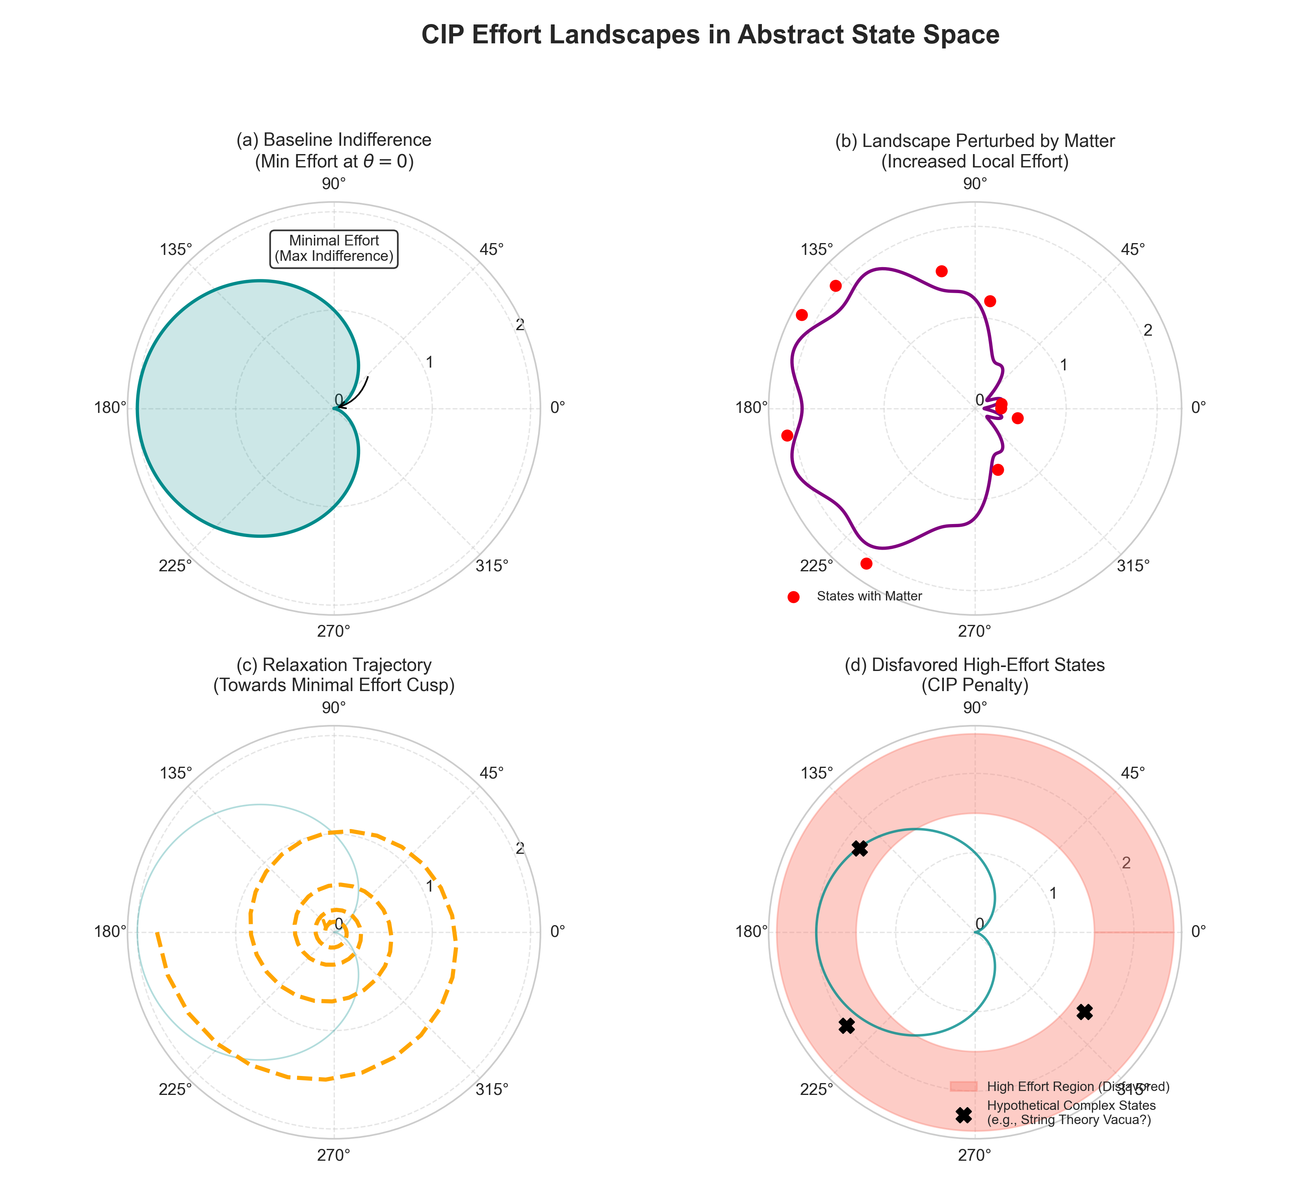
\includegraphics[width=\textwidth]{CIP_StateSpace.png}
    \caption[CIP Effort Landscapes in Abstract State Space]{CIP Effort Landscapes in Abstract State Space. (a) Baseline Indifference: Minimal effort at $\theta=0$ (representing $\Phi_{\subt{CIP}}=0$). (b) Landscape Perturbed by Matter: Presence of matter (red dots) increases local effort, perturbing the landscape. (c) Relaxation Trajectory: Systems naturally spiral towards the minimal effort cusp. (d) Disfavored High-Effort States: Regions requiring high specification (high effort penalty, e.g., hypothetical complex states like String Theory Vacua?) are ontologically disfavored.}
    \label{fig:state_space}
\end{figure}


\subsection{CIP in Contrast: Critiquing Scientific Theories}

\begin{enumerate}
    \item \textbf{Quantum Superposition:} Not simultaneous states, but refusal of effort to settle until forced. Profound pre-measurement indifference.
    \item \textbf{GR's Singularities:} Not portals, but artefacts where theory demands infinite effort/specification, which CIP prohibits.
    \item \textbf{Standard Model Menagerie:} Are all particles equally fundamental? Perhaps some are lower-effort configs, others transient excitations tolerated briefly before decay (indifference reasserts).
    \item \textbf{String Theory's Landscape:} Landscape of $10^{500}$ vacua? Prodigious cataloguing effort aside, complex Calabi-Yau geometries demand high specification cost (high structured $\Phi_{\subt{CIP}}$). CIP argues against such intrinsic manipulations. Why assume trillions of pre-designed castles? Default is scattered pile or undifferentiated soup. Landscape seems testament to theoretical over-enthusiasm, not reality. CIP suggests one baseline indifference ($\Phi_{\subt{CIP}}=0$) and maybe few shallow depressions.
    \item \textbf{Cosmic Inflation:} Complex inflaton field vs. universe simply starting smooth because homogeneity requires less specification effort? Why invent elaborate flattening machine?
    \item \textbf{Maxwell's Demon & 2nd Law:} Paradox only if information is free. CIP: Info requires effort, cost outweighs local gain. 2nd Law = universe enforcing budget.
    \item \textbf{Biological Evolution & Complexity:} Life not cosmic drive, but frantic cascade surfing energy gradients, locally counteracting pull to equilibrium. Desperate fight *against* CIP's preferred state.
    \item \textbf{Information Theory & Kolmogorov:} Crucial measure not description length, but *effort for state to persist*. High-entropy gas requires near-zero effort *to be*. CIP measures existential exertion.
    \item \textbf{GR-QM Conflict:} Not deep flaw, but consequence of stapling regimes of different effort. GR=costly spacetime sculpting; QM=minimal-effort content antics. Clash because underlying cost mediator (CIP) ignored.
    \item \textbf{Symmetry Principles:} Often arise not from deep design, but profound *indifference*. Isotropic state requires minimal specification. Symmetry = face of non-commitment.
    \item \textbf{Holographic Principle:} Encoding volume info on boundary? Immense specification density on surface seems profoundly wasteful (high local $\Phi_{\subt{CIP}}$). Akin to etching brick states on walls. Contrary to indifference favoring information dissipation. Holography seems attempt to impose max info retention on universe striving for minimal specification.
\end{enumerate}


\subsection{Reinterpreting Simplicity, Cost, and Structure} \label{sec:reinterpreting}

The rigorous application of CIP, particularly the understanding that maximal entropy represents radical simplicity via minimal definition cost (Sec.~\ref{sec:entropy_complexity}), leads to several counter-intuitive yet unavoidable conclusions:

\begin{enumerate}
    \item \textbf{The Ontological Cheapness of the Pile:} Is the disordered pile of Lego bricks truly simpler and lower cost than maintaining the bricks as distinct entities? \textbf{Yes.} Minimizing $V(\Phi_{\subt{CIP}})$ favors reducing relational information and boundary definitions. Less active specification *is* fundamentally simpler/cheaper. Maximal entropy is ontologically favored due to minimal definitional burden.

    \item \textbf{Redefining "Primitive"; Complexity Under Duress:} Could a complex structure, like the LHC replica, ever be considered a more "primitive" or lower-effort state under CIP? \textbf{Intrinsically, no. Conditionally, perhaps.} The \textit{static* configuration is high-effort ($\Phi_{\subt{CIP}}$). However, dynamics follow least effort *processes* under constraints. If forced (e.g., massive energy influx, specific boundary conditions), forming a transient complex structure *might* be the momentarily lowest-effort *pathway* to dissipate energy or satisfy constraints (like eddies in turbulence). It's "primitive" only as an unavoidable intermediate response *under duress*, before inevitable relaxation. Crucial distinction: cost of \textit{state} vs. cost of \textit{process* under constraint.

    \item \textbf{Information as Burden:} CIP reframes information not as resource, but as *burden* with ontological cost. Universe seeks to shed this via entropy increase (dissolving specificity). Knowledge/structure are expensive deviations from ignorant bliss.

    \item \textbf{The Ambiguous Cost of Replication:} Is building a replica (Lego LHC) cheaper than original via templating? \textbf{Profoundly ambiguous.}
    \begin{itemize}
        \item \textit{Reduced Effort Argument (Process Efficiency):} Templating bypasses \textit{de novo} specification. "Design" effort paid. Replication follows pattern (cf. biology, crystal growth). Might be CIP-permitted mechanism for costly states via less-costly *process*, especially under energy flux. Template lowers barrier.
        \item \textit{Against Reduced Effort Argument (State Cost Dominance):} Replica's *final state* has identical high complexity, same high sustained $\Phi_{\subt{CIP}}$, same $V(\Phi_{\subt{CIP}})$ penalty. CIP penalizes the *existence* of specified states. Replication *process* itself also costs effort (reading template, assembly, error-correction). Is saving on initial specification > cost of replication + final state penalty?
        \item \textit{Provocative Implication:} Life (replication-based) exists precariously. Exploits efficient templating *processes* (loophole under energy flux?) but perpetually fights high $V(\Phi_{\subt{CIP}})$ cost of its own complex *state*. Frantic, temporary exploitation of process efficiency, forever subject to dissolution drive imposed by high ontological cost. Less cheating CIP, more finding least exhausting temporary resistance.
    \end{itemize}
\end{enumerate}

These corollaries underscore the radical shift demanded by CIP. Simplicity, cost, physical law re-evaluated through austere lens of minimal necessary effort and specification.


% --- Conclusion ---
\section{Conclusion: Embrace Indifference} \label{sec:conclusion}

Modern physics is paradigms ridden. The solution is simple: The \textbf{Cosmic Indifference Principle (CIP)}. The universe defaults to minimal effort.

CIP, via $\Phi_{\subt{CIP}}$ and $L_{\subt{CIP}}$, unifies physics parsimoniously. Quantum mechanics, cosmology, thermodynamics become consequences of cosmic apathy (Sec.~\ref{sec:explanations}). Predictions favor simplicity and null results against complex models (Sec.~\ref{sec:predictions}). Occam's Razor becomes ontological imperative (Sec.~\ref{sec:discussion}).

Abandon anthropocentric bias. Accept randomness and equilibrium as fundamental. Strip away theoretical epicycles. Future work: refine $L_{\subt{CIP}}$ parameters, apply to quantum gravity (resolves singularities), critique complex programs via CIP.
CIP's success is often measured by what doesn't happen, aligning with its principle of minimal necessary action. Often theories are valued on what they predict. But this theory is also maximally successful in what it does \textit{not} predict.
Progress lies in recognizing universal thermodynamic apathy. CIP is the foundational principle. The universe is indifferent. Physics should follow. Effort saved will be significant.

\clearpage

% --- Appendix / Addendum ---
\appendix % Or use \section*{...} for unnumbered section
\section{Mathematical Addendum: On the Ineluctable Efficiency of Complex Numbers as Evidence for CIP Incomplexity}

A persistent feature of fundamental physics, particularly quantum mechanics, is the apparently indispensable role of complex numbers ($\mathbb{C}$). This has often been treated either as a mere calculational convenience or a deep mystery hinting at hidden realities. From the perspective of Cosmic Indifference, however, the necessity of $\mathbb{C}$ is neither convenience nor mystery; it is a direct, almost trivial consequence of the principle of minimal configurational effort.

\textbf{Premise:} The Cosmic Indifference Principle (CIP) mandates that physical states and their evolution minimize 'attentiveness cost,' equivalent to minimizing unnecessary specification or configurational burden.

\textbf{Consider:} A fundamental quantum state, prior to measurement, exists in a condition of baseline indifference regarding certain classical observables (e.g., definite position \textit{and} momentum). Yet, it possesses quantifiable potentiality (amplitude) and crucial relational information (phase). Let this state be represented by $\psi$.

\textbf{The Representational Mandate:} What is the minimal mathematical structure capable of encoding both amplitude ($r$) and relative phase ($\theta$) without imposing premature classical specification and without demanding extraneous descriptive elements?

\textbf{Proposition:} The field of complex numbers, $\mathbb{C}$, provides this unique minimal structure.

\textbf{Demonstration:}

\begin{enumerate}
    \item \textbf{Encoding Amplitude and Phase:} A complex number $z = r e^{i\theta}$ elegantly packages precisely two essential degrees of freedom: magnitude $r$ (related to probability amplitude) and phase $\theta$. This representation, via Euler's identity ($e^{i\theta} = \cos(\theta) + i \sin(\theta)$), implicitly uses the orthogonal dimensions of the complex plane ($a + bi$) to achieve this minimal encoding.

    \item \textbf{Avoiding Real-Valued Overhead:} Attempting to represent $\psi$ using only real numbers ($\mathbb{R}$) necessitates \textit{more} structure, not less. One would require \textit{two* independent real-valued functions (e.g., $\psi_{\subt{real}}(x,t)$ and $\psi_{\subt{imaginary}}(x,t)$, or explicit $\mathrm{Amplitude}(x,t)$ and $\mathrm{Phase}(x,t)$ functions). This introduces descriptive redundancy or forces a separation of intrinsically linked properties, incurring unwarranted 'configurational effort'—a violation of CIP's mandate for ontological parsimony.

    \item \textbf{Minimal Specification via $i$:} The imaginary unit $i$ is not an indicator of 'unreality'. It is the minimal mathematical operator required to introduce the necessary orthogonal dimension (phase) relative to amplitude without imposing additional structure. It is the most efficient notation for the state's inherent indifference to possessing purely 'real' classical properties before interaction.

    \item \textbf{Effortless Probability Extraction:} The extraction of observable probability, necessitated by measurement (an interaction forcing specification), is achieved via the modulus squared operation: $P = |\psi|^2 = \psi^*\psi$. This operation is \textit{intrinsic* to the algebra of complex numbers. It requires no additional postulates or mechanisms; it is the most direct, mathematically 'low-effort' method to yield a real, positive value (probability) from the state description $\psi$. A purely real formalism would require a more contrived operation to guarantee positivity and link the descriptive components to probability.

    \item \textbf{Phase Invariance and Indifference:} The physical irrelevance of a global phase factor ($\psi$ vs $e^{i\alpha}\psi$) is naturally accommodated within $\mathbb{C}$. The modulus $|\psi|$ is invariant under such transformations. This mathematical 'gauge freedom' directly mirrors CIP: the universe is indifferent to, and expends no effort maintaining, absolute phase information that lacks relational significance. Complex numbers inherently possess this 'indifferent' property.
\end{enumerate}

\textbf{Complex Number Proof Conclusion:}

The mandatory emergence of complex numbers in our most fundamental description of reality (QM) is not a sign of nature's complexity, but compelling evidence of its adherence to \textbf{minimal configurational effort}. The complex structure $\mathbb{C}$ is the uniquely efficient mathematical language required to describe states adhering to CIP – states possessing both amplitude and relative phase while remaining indifferent to premature classical specification. The universe utilizes complex numbers because doing so represents the path of least descriptive resistance, the most economical way to structure its fundamental indifference. To insist on purely real descriptions would be mathematically less efficient and thus, according to CIP, physically prohibited. The structure of $\mathbb{C}$ \textit{is} the structure of minimal ontological effort made manifest in mathematics.

% --- Bibliography ---
\clearpage
\bibliographystyle{plain} % Or another suitable style like 'unsrt', 'abbrv', 'ieeetr'
\bibliography{references}  % Assumes references.bib file in the same directory

\end{document}